% Options for packages loaded elsewhere
\PassOptionsToPackage{unicode}{hyperref}
\PassOptionsToPackage{hyphens}{url}
%
\documentclass[
]{book}
\usepackage{lmodern}
\usepackage{amsmath}
\usepackage{ifxetex,ifluatex}
\ifnum 0\ifxetex 1\fi\ifluatex 1\fi=0 % if pdftex
  \usepackage[T1]{fontenc}
  \usepackage[utf8]{inputenc}
  \usepackage{textcomp} % provide euro and other symbols
  \usepackage{amssymb}
\else % if luatex or xetex
  \usepackage{unicode-math}
  \defaultfontfeatures{Scale=MatchLowercase}
  \defaultfontfeatures[\rmfamily]{Ligatures=TeX,Scale=1}
  \setmainfont[]{NanumMyeongjo}
\fi
% Use upquote if available, for straight quotes in verbatim environments
\IfFileExists{upquote.sty}{\usepackage{upquote}}{}
\IfFileExists{microtype.sty}{% use microtype if available
  \usepackage[]{microtype}
  \UseMicrotypeSet[protrusion]{basicmath} % disable protrusion for tt fonts
}{}
\makeatletter
\@ifundefined{KOMAClassName}{% if non-KOMA class
  \IfFileExists{parskip.sty}{%
    \usepackage{parskip}
  }{% else
    \setlength{\parindent}{0pt}
    \setlength{\parskip}{6pt plus 2pt minus 1pt}}
}{% if KOMA class
  \KOMAoptions{parskip=half}}
\makeatother
\usepackage{xcolor}
\IfFileExists{xurl.sty}{\usepackage{xurl}}{} % add URL line breaks if available
\IfFileExists{bookmark.sty}{\usepackage{bookmark}}{\usepackage{hyperref}}
\hypersetup{
  pdftitle={{[}UST 2021{]} 데이터 사이언스를 위한 R 프로그래밍},
  pdfauthor={한국생명공학연구원 김하성},
  hidelinks,
  pdfcreator={LaTeX via pandoc}}
\urlstyle{same} % disable monospaced font for URLs
\usepackage{color}
\usepackage{fancyvrb}
\newcommand{\VerbBar}{|}
\newcommand{\VERB}{\Verb[commandchars=\\\{\}]}
\DefineVerbatimEnvironment{Highlighting}{Verbatim}{commandchars=\\\{\}}
% Add ',fontsize=\small' for more characters per line
\usepackage{framed}
\definecolor{shadecolor}{RGB}{248,248,248}
\newenvironment{Shaded}{\begin{snugshade}}{\end{snugshade}}
\newcommand{\AlertTok}[1]{\textcolor[rgb]{0.94,0.16,0.16}{#1}}
\newcommand{\AnnotationTok}[1]{\textcolor[rgb]{0.56,0.35,0.01}{\textbf{\textit{#1}}}}
\newcommand{\AttributeTok}[1]{\textcolor[rgb]{0.77,0.63,0.00}{#1}}
\newcommand{\BaseNTok}[1]{\textcolor[rgb]{0.00,0.00,0.81}{#1}}
\newcommand{\BuiltInTok}[1]{#1}
\newcommand{\CharTok}[1]{\textcolor[rgb]{0.31,0.60,0.02}{#1}}
\newcommand{\CommentTok}[1]{\textcolor[rgb]{0.56,0.35,0.01}{\textit{#1}}}
\newcommand{\CommentVarTok}[1]{\textcolor[rgb]{0.56,0.35,0.01}{\textbf{\textit{#1}}}}
\newcommand{\ConstantTok}[1]{\textcolor[rgb]{0.00,0.00,0.00}{#1}}
\newcommand{\ControlFlowTok}[1]{\textcolor[rgb]{0.13,0.29,0.53}{\textbf{#1}}}
\newcommand{\DataTypeTok}[1]{\textcolor[rgb]{0.13,0.29,0.53}{#1}}
\newcommand{\DecValTok}[1]{\textcolor[rgb]{0.00,0.00,0.81}{#1}}
\newcommand{\DocumentationTok}[1]{\textcolor[rgb]{0.56,0.35,0.01}{\textbf{\textit{#1}}}}
\newcommand{\ErrorTok}[1]{\textcolor[rgb]{0.64,0.00,0.00}{\textbf{#1}}}
\newcommand{\ExtensionTok}[1]{#1}
\newcommand{\FloatTok}[1]{\textcolor[rgb]{0.00,0.00,0.81}{#1}}
\newcommand{\FunctionTok}[1]{\textcolor[rgb]{0.00,0.00,0.00}{#1}}
\newcommand{\ImportTok}[1]{#1}
\newcommand{\InformationTok}[1]{\textcolor[rgb]{0.56,0.35,0.01}{\textbf{\textit{#1}}}}
\newcommand{\KeywordTok}[1]{\textcolor[rgb]{0.13,0.29,0.53}{\textbf{#1}}}
\newcommand{\NormalTok}[1]{#1}
\newcommand{\OperatorTok}[1]{\textcolor[rgb]{0.81,0.36,0.00}{\textbf{#1}}}
\newcommand{\OtherTok}[1]{\textcolor[rgb]{0.56,0.35,0.01}{#1}}
\newcommand{\PreprocessorTok}[1]{\textcolor[rgb]{0.56,0.35,0.01}{\textit{#1}}}
\newcommand{\RegionMarkerTok}[1]{#1}
\newcommand{\SpecialCharTok}[1]{\textcolor[rgb]{0.00,0.00,0.00}{#1}}
\newcommand{\SpecialStringTok}[1]{\textcolor[rgb]{0.31,0.60,0.02}{#1}}
\newcommand{\StringTok}[1]{\textcolor[rgb]{0.31,0.60,0.02}{#1}}
\newcommand{\VariableTok}[1]{\textcolor[rgb]{0.00,0.00,0.00}{#1}}
\newcommand{\VerbatimStringTok}[1]{\textcolor[rgb]{0.31,0.60,0.02}{#1}}
\newcommand{\WarningTok}[1]{\textcolor[rgb]{0.56,0.35,0.01}{\textbf{\textit{#1}}}}
\usepackage{longtable,booktabs}
\usepackage{calc} % for calculating minipage widths
% Correct order of tables after \paragraph or \subparagraph
\usepackage{etoolbox}
\makeatletter
\patchcmd\longtable{\par}{\if@noskipsec\mbox{}\fi\par}{}{}
\makeatother
% Allow footnotes in longtable head/foot
\IfFileExists{footnotehyper.sty}{\usepackage{footnotehyper}}{\usepackage{footnote}}
\makesavenoteenv{longtable}
\usepackage{graphicx}
\makeatletter
\def\maxwidth{\ifdim\Gin@nat@width>\linewidth\linewidth\else\Gin@nat@width\fi}
\def\maxheight{\ifdim\Gin@nat@height>\textheight\textheight\else\Gin@nat@height\fi}
\makeatother
% Scale images if necessary, so that they will not overflow the page
% margins by default, and it is still possible to overwrite the defaults
% using explicit options in \includegraphics[width, height, ...]{}
\setkeys{Gin}{width=\maxwidth,height=\maxheight,keepaspectratio}
% Set default figure placement to htbp
\makeatletter
\def\fps@figure{htbp}
\makeatother
\setlength{\emergencystretch}{3em} % prevent overfull lines
\providecommand{\tightlist}{%
  \setlength{\itemsep}{0pt}\setlength{\parskip}{0pt}}
\setcounter{secnumdepth}{5}
\usepackage{booktabs}
\ifluatex
  \usepackage{selnolig}  % disable illegal ligatures
\fi
\usepackage[]{natbib}
\bibliographystyle{apalike}

\title{{[}UST 2021{]} 데이터 사이언스를 위한 R 프로그래밍}
\author{한국생명공학연구원 김하성}
\date{2021-03-04}

\begin{document}
\maketitle

{
\setcounter{tocdepth}{1}
\tableofcontents
}
\hypertarget{introduction-uxac15uxc758-uxac1cuxc694}{%
\chapter{Introduction 강의 개요}\label{introduction-uxac15uxc758-uxac1cuxc694}}

\begin{itemize}
\tightlist
\item
  매주 목요일 강의노트, 동영상 업데이트
\item
  강사: 한국생명공학연구원 바이오합성연구센터 김하성
\item
  연락처: 042-860-4372, haseong {[}at{]} kribb.re.kr (생명연 연구동 1143)
\item
  강의조교: 박성군, tjdrns27 {[}at{]} kribb.re.kr
\item
  강의site: \url{https://greendaygh.github.io/Rprog2021/}
\end{itemize}

\hypertarget{goal-uxac15uxc758-uxbaa9uxd45c}{%
\section{Goal 강의 목표}\label{goal-uxac15uxc758-uxbaa9uxd45c}}

\begin{itemize}
\tightlist
\item
  이공계열 대학원생이 그들의 원활한 실험 설계와 데이터 분석을 위해 범용 프로그램 언어인 R의 사용법과 프로그래밍 기술을 습득할수 있도록 하는데 목표가 있음. 특히 Data scientist를 위해 개발된 tidyverse 패키지 위주의 강의를 진행함.
\end{itemize}

\hypertarget{this-course}{%
\section{This course}\label{this-course}}

\begin{itemize}
\tightlist
\item
  이 강좌는 온라인 (강의자료, 동영상) 강의를 기본으로 함
\item
  R에 대한 기본 개념과 사용법, 데이터분석 중심의 설명, 필요시 기초 통계 지식 강의
\item
  매회 강의에는 해당 강의 내용과 관련된 과제가 주어지며 이메일을 통해 문제 풀이를 제출받음
\item
  상황에 따라 강의자료 및 동영상 업데이트 일정이 조정될 수 있음
\item
  \textbf{참고} 온라인 강의 특성상 스스로 학습하려는 의지가 강하지 않으면 효과가 없습니다. 매시간 작은 것이라도 배워간다는 마음으로 강의에 임해주시기 바랍니다
\end{itemize}

\hypertarget{tips}{%
\section{Tips}\label{tips}}

\begin{itemize}
\tightlist
\item
  눈으로 이해하지 않고 스스로 실습 필수
\item
  각 명령줄이 어떻게/왜 작동하는지 이해하기
\item
  인터넷 검색을 통한 다른사람의 코드 이해/적용 필요
\end{itemize}

\hypertarget{references-books-uxc8fcuxc694uxcc38uxace0-uxad50uxc81c}{%
\section{References books 주요/참고 교제}\label{references-books-uxc8fcuxc694uxcc38uxace0-uxad50uxc81c}}

\begin{itemize}
\tightlist
\item
  R for Data Science (\url{https://r4ds.had.co.nz}, \url{https://github.com/hadley})
\item
  Hands-On Programming with R (\url{https://rstudio-education.github.io/hopr/})
\item
  Using R for Introductory Statistics by John Verzani

  \begin{itemize}
  \tightlist
  \item
    Free version of 1st Edition

    \begin{itemize}
    \tightlist
    \item
      \url{https://cran.r-project.org/doc/contrib/Verzani-SimpleR.pdf}
    \end{itemize}
  \item
    Second edition

    \begin{itemize}
    \tightlist
    \item
      \url{https://www.crcpress.com/Using-R-for-Introductory-Statistics-Second-Edition/Verzani/p/book/9781466590731}
    \end{itemize}
  \end{itemize}
\item
  Bioinformatics Data Skills by Vince Buffalo (\url{http://2.droppdf.com/files/5aTvl/bioinformatics-data-skills.pdf})
\item
  First Course in Statistical Programming with R by Braun and
  Murdoch (\url{https://www.cambridge.org/core/books/first-course-in-statistical-programming-with-r/C9F088122AB40517B07FA77F2F0FDE2F})
\item
  Introductory Statistics with R by Dalgaard (\url{http://www.academia.dk/BiologiskAntropologi/Epidemiologi/PDF/Introductory_Statistics_with_R__2nd_ed.pdf})
\item
  Modern Applied Statistics with S by Venables and Ripley (\url{http://www.bagualu.net/wordpress/wp-content/uploads/2015/10/Modern_Applied_Statistics_With_S.pdf})
\item
  일반통계학 (영지문화사, 김우철 외)
\end{itemize}

\hypertarget{references-uxcc38uxace0-uxc790uxb8cc}{%
\section{References 참고 자료}\label{references-uxcc38uxace0-uxc790uxb8cc}}

\begin{itemize}
\tightlist
\item
  \url{https://resources.rstudio.com/}
\item
  \url{http://shiny.rstudio.com/tutorial/}
\item
  R 홈페이지 \url{https://www.r-project.org/}
\item
  Rstudio 홈페이지 \url{https://www.rstudio.com/}
\item
  Packages for biologists \url{https://www.bioconductor.org/}
\item
  R 기본 문서들 (소개, 사용, 설치, 운영) \url{https://cran.r-project.org/manuals.html}
\item
  R ebooks \url{https://bookdown.org/}
\item
  Cheat Sheets \url{https://www.rstudio.com/resources/cheatsheets/}
\end{itemize}

\hypertarget{evaluation-uxd3c9uxac00-uxc138uxbd80-uxd56duxbaa9}{%
\section{Evaluation 평가 세부 항목}\label{evaluation-uxd3c9uxac00-uxc138uxbd80-uxd56duxbaa9}}

\begin{itemize}
\item
  과제 100\%
\item
  성적부여기준: 최종 평균균 70점 이상 S, 70점 미만 U 부여
\item
  과제 채점: 각 과제당 총점 100점 만점 환산 점수 (답이 틀려도 코드가 있으면 가산점)
\item
  과제 제출일: 수업 자료 배포 후 1주일 (목요일 강의 자료 배포 -\textgreater{} 그 다음주 목요일 까지)
\item
  과제 솔루션 배포: 과제 제출일 마감 이 후 조교 배포
\item
  감점 기준

  \begin{itemize}
  \tightlist
  \item
    과제 제출일 (1주) 이내 제출: 감점 없음
  \item
    과제 제출일 (1주) 이후 제출: 20점 감점
  \item
    솔루션 배포 이후 과제 제출: 40점 감점\\
  \item
    과제 미제출: 100점 감점
  \item
    참고로 S/U 판단은 최종 평가시 평균 70정으로 진행행
  \end{itemize}
\end{itemize}

\hypertarget{schedule-uxac15uxc758-uxacc4uxd68d}{%
\section{Schedule 강의 계획}\label{schedule-uxac15uxc758-uxacc4uxd68d}}

\begin{itemize}
\tightlist
\item
  1주차 - R basics / introduction of data
\item
  2주차 - Univariate data -- Summary statistics
\item
  3주차 - Bivariate data -- Correlation / Independence\\
\item
  4주차 - Multivariate data -- R data structure
\item
  5주차 - Populations -- Families of distributions
\item
  6주차 - Sampling -- Distribution and CLT
\item
  7주차 - Statistical inference
\item
  8주차 - Confidence intervals
\item
  9주차 - Significance test - parameteric
\item
  10주차 - Significance test -- non parametric
\item
  11주차 - Goodness of fit - parametric
\item
  12주차 - Goodness of fit -- non parametirc
\item
  13주차 - Linear regression -- basics \& simple LR
\item
  14주차 - Multiple linear regression
\item
  15주차 - Analysis of variance
\item
  16주차 - Logistic / Non-linear regression
\end{itemize}

\hypertarget{r-lecture-youtube-link}{%
\section{R Lecture Youtube Link}\label{r-lecture-youtube-link}}

\hypertarget{lecture-chapter-1}{%
\subsection{Lecture Chapter 1}\label{lecture-chapter-1}}

\hypertarget{lecture-2}{%
\subsection{Lecture 2}\label{lecture-2}}

\hypertarget{lecture-3}{%
\subsection{Lecture 3}\label{lecture-3}}

\hypertarget{lecture-4}{%
\subsection{Lecture 4}\label{lecture-4}}

\hypertarget{lecture-5}{%
\subsection{Lecture 5}\label{lecture-5}}

\hypertarget{lecture-6}{%
\subsection{Lecture 6}\label{lecture-6}}

\hypertarget{lecture-7}{%
\subsection{Lecture 7}\label{lecture-7}}

\hypertarget{r-basics}{%
\chapter{R basics}\label{r-basics}}

\hypertarget{what-is-r-rstudio}{%
\section{What is R / Rstudio}\label{what-is-r-rstudio}}


\includegraphics{images/01/r.jpg}

R은 통계나 생물통계, 유전학을 연구하는 사람들 사이에서 널리 사용되는 오픈소스 프로그래밍 언어 입니다. Bell Lab에서 개발한 S 언어에서 유래했으며 엄청나게 많은 라이브러리 (다른 사람들이 만들어 놓은 코드)가 있어서 쉽게 가져다 사용할 수 있습니다. R은 복잡한 수식이나 통계 알고리즘을 간단히 구현하고 사용할 수 있으며 C, C++, Python 등 다른 언어들과의 병행 사용도 가능합니다. 2019년 top five language에 랭크 되었으며 이는 빅데이터 증가에 따라 인기가 높아진 것으로 볼 수 있습니다 (참고로 2018년에는 7위).

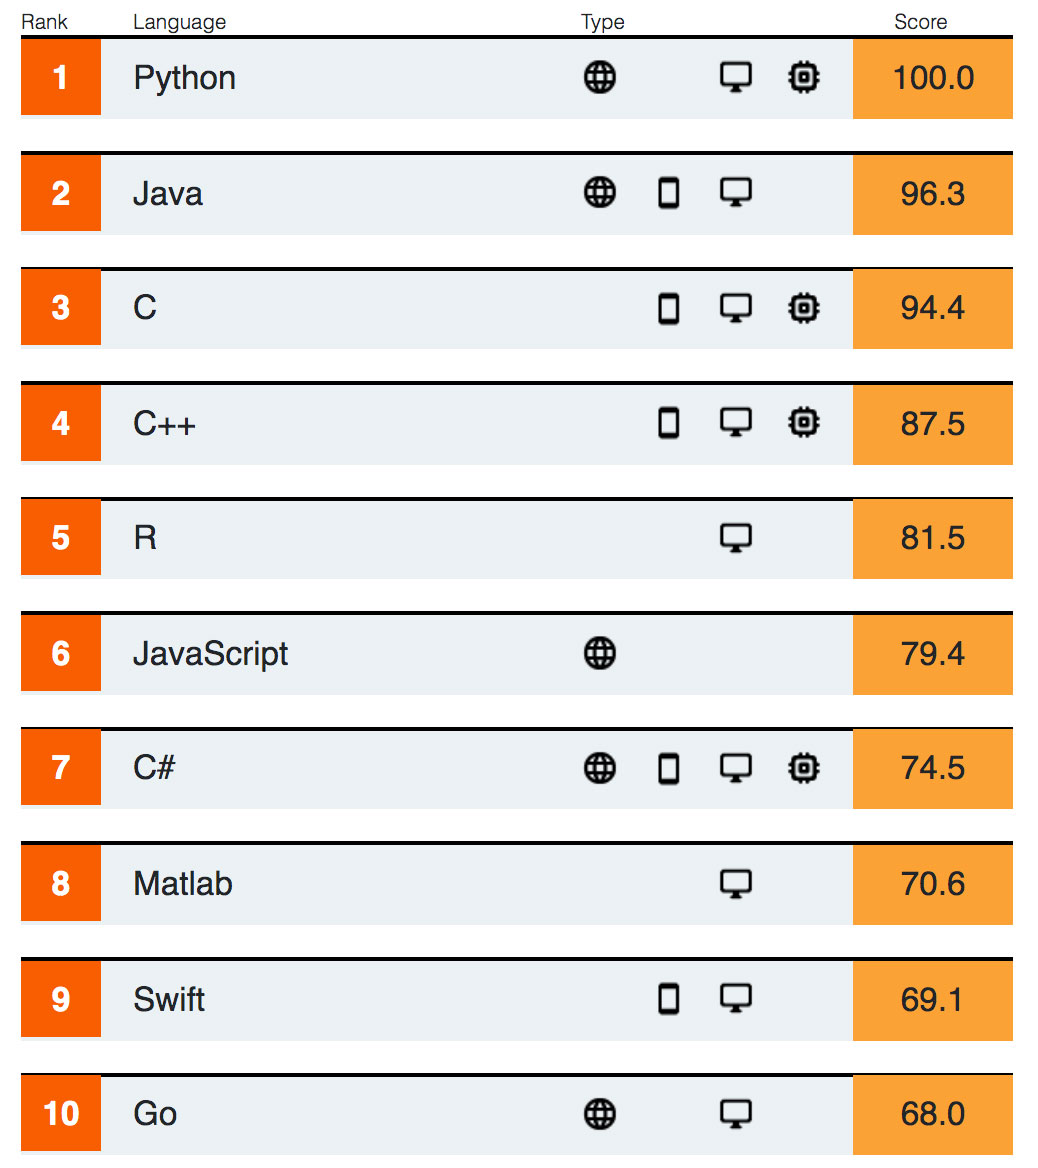
\includegraphics[width=4.6875in,height=\textheight]{images/01/topproglang.jpeg}

Despite being a much more specialized language than the others, it's maintained its popularity in recent years due to the world being awash in an ever-growing pile of big data.
\url{https://spectrum.ieee.org/computing/software/the-top-programming-languages-2019}

R은 데이터를 통계분석에 널리 사용되는데 이는 데이터를 눈으로 확인하기 위한 visualization 이나 벡터 연산 등의 강력한 기능 때문에 점점 더 많은 사람들이 사용하고 있습니다. 기존에는 속도나 확장성이 다른 언어들에 비해 단점으로 지적되었으나 R 언어의 계속적인 개발과 업데이트로 이러한 단점들이 빠르게 보완되고 있습니다. R 사용을 위해서는 R 언어의 코어 프로그램을 먼저 설치하고 그 다음 R 언어용 IDE인 RStudio 설치가 필요합니다.

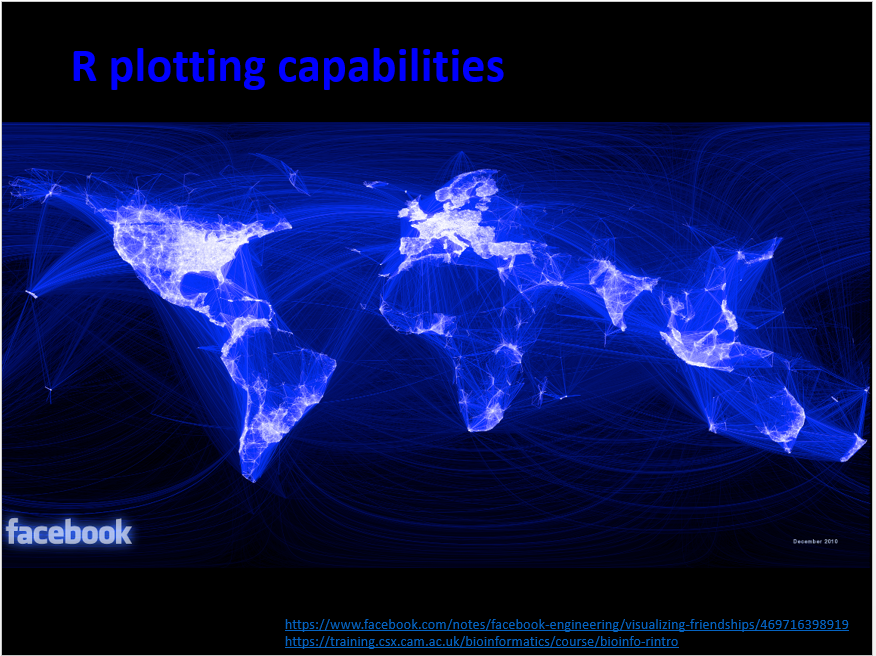
\includegraphics{images/01/22.PNG}

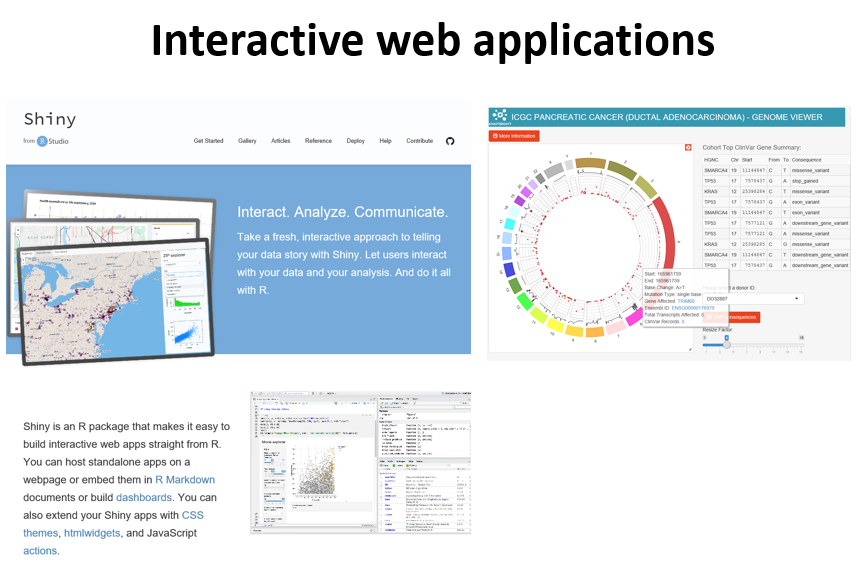
\includegraphics{images/01/23.PNG}

\hypertarget{r-rstudio-installation}{%
\section{R / Rstudio installation}\label{r-rstudio-installation}}

\begin{itemize}
\item
  R 사이트에 접속 후 (\url{https://www.r-project.org/}) 좌측 메뉴 상단에 위치한 CRAN 클릭.
  
\includegraphics{images/01/01-01.PNG}
\item
  미러 사이트 목록에서 Korea의 아무 사이트나 들어감
  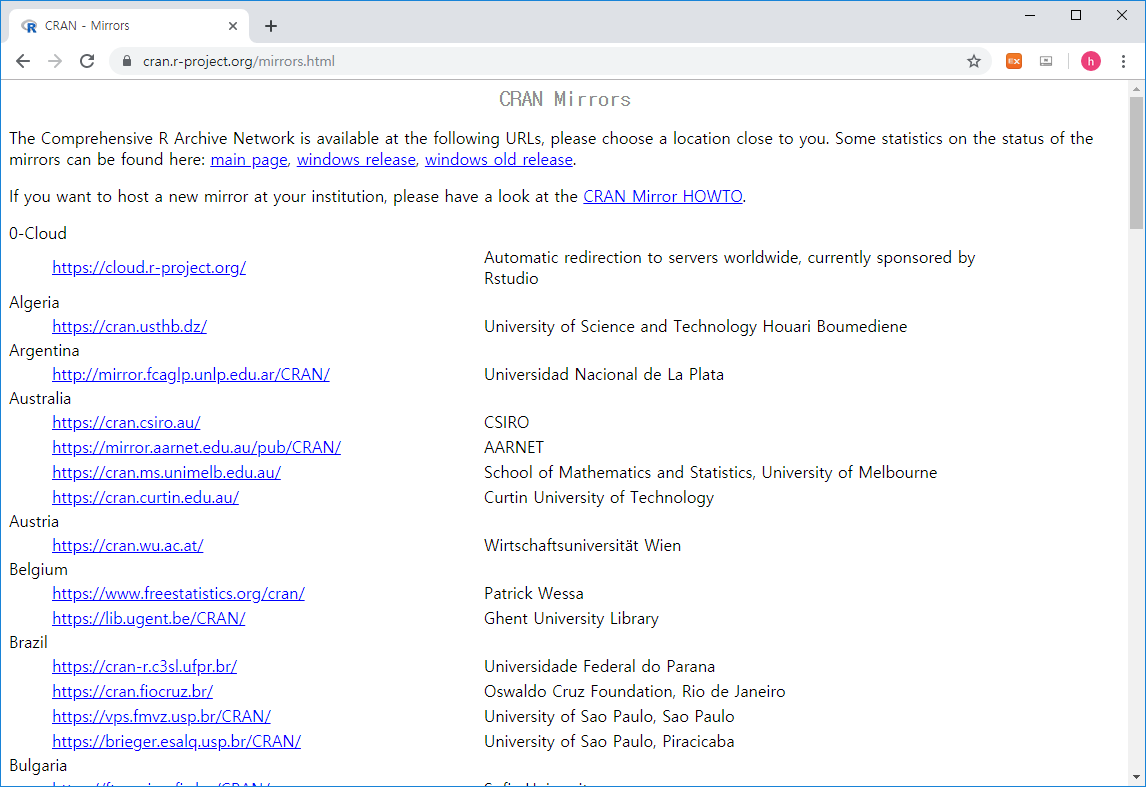
\includegraphics{images/01/01-02.PNG}
\item
  Download R for Windows를 클릭 후 base 링크 들어가서
  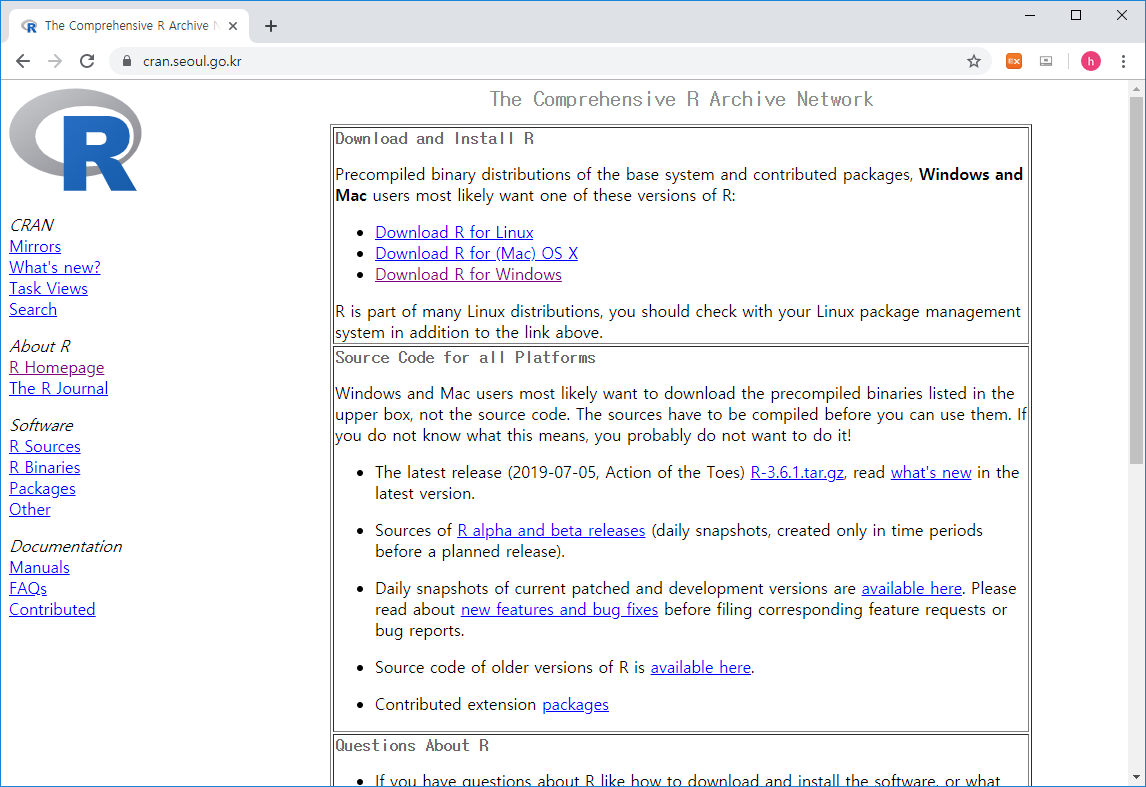
\includegraphics{images/01/01-03.PNG}\\
  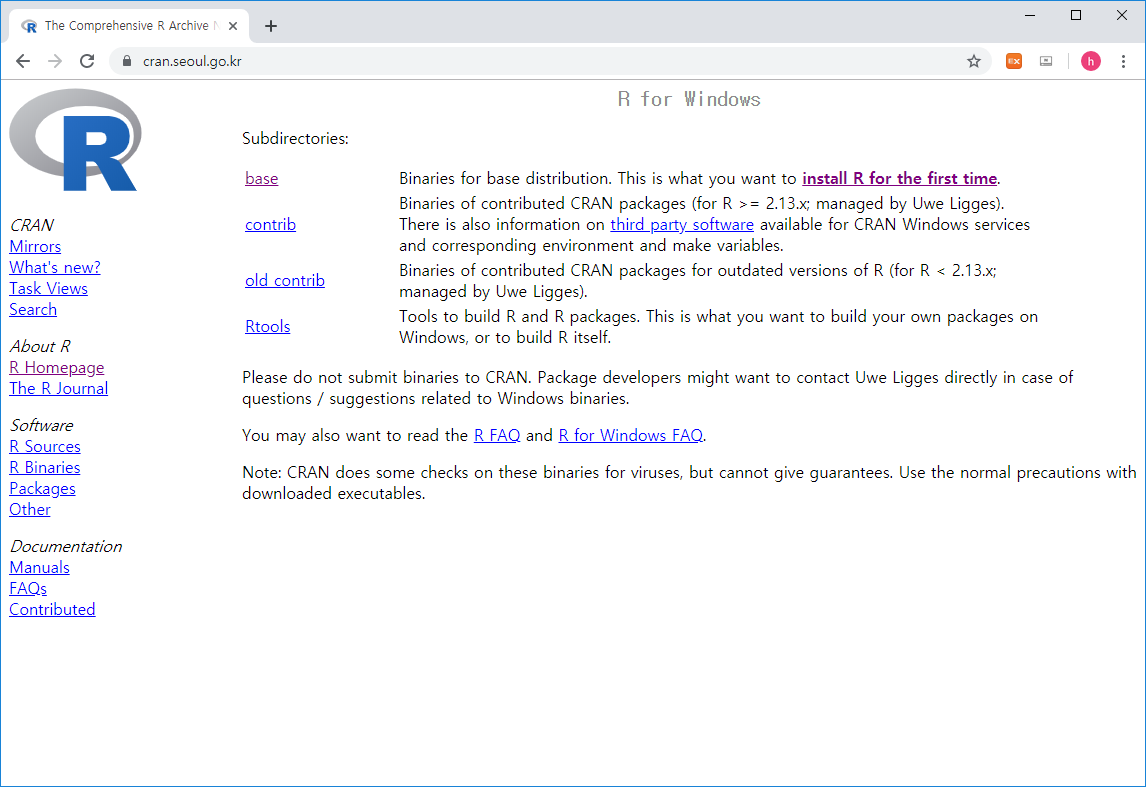
\includegraphics{images/01/01-04.PNG}
\item
  Download R 3.6.3 for Windows 링크로 실행 프로그램 다운로드 (2020.3 현재 R 버전은 3.6.3). 로컬 컴퓨터에 Download 된 R-3.6.3-win.exe 를 실행하고 설치 프로그램의 지시에 따라 R 언어 소프트웨어 설치를 완료합니다.
\end{itemize}

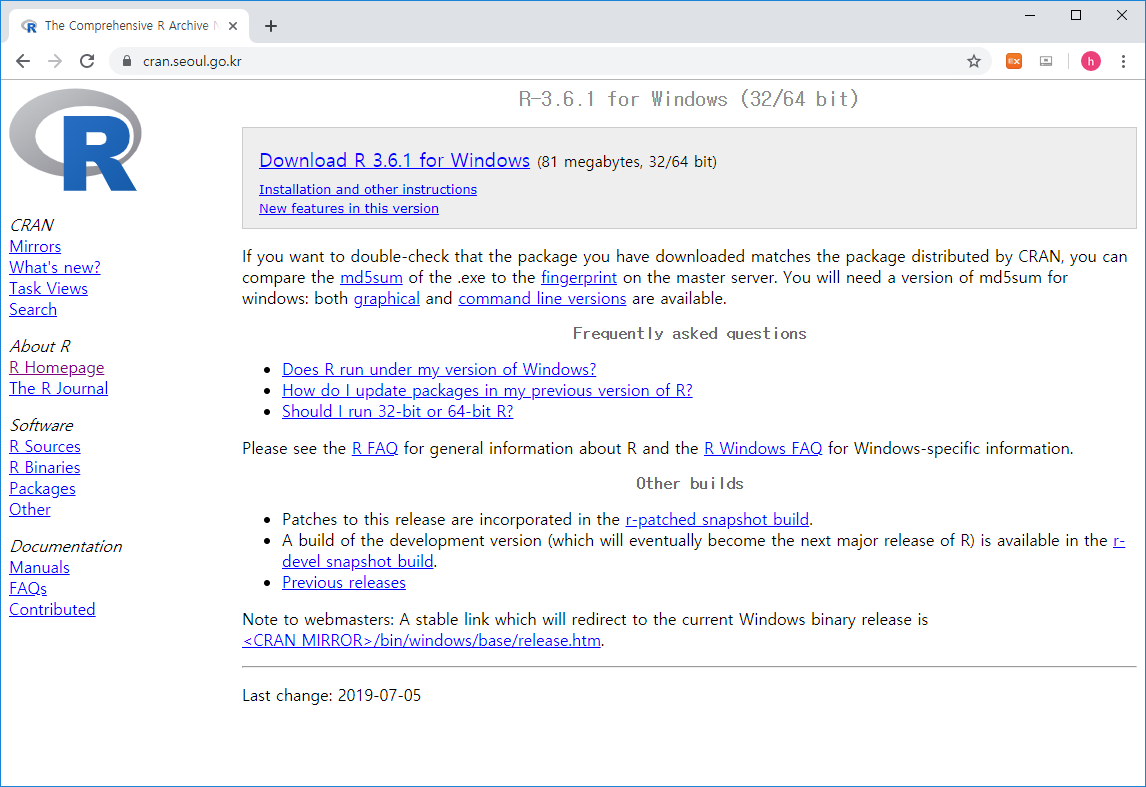
\includegraphics{images/01/01-05.PNG}

\begin{itemize}
\item
  Rstudio는 R 언어를 위한 오픈소스 기반 통합개발환경(IDE)으로 R 프로그래밍을 위한 편리한 기능들을 제공해 줍니다. 다음 사이트에 접속 (\url{https://www.rstudio.com/}), 상단의 Products \textgreater{} RStudio 클릭
  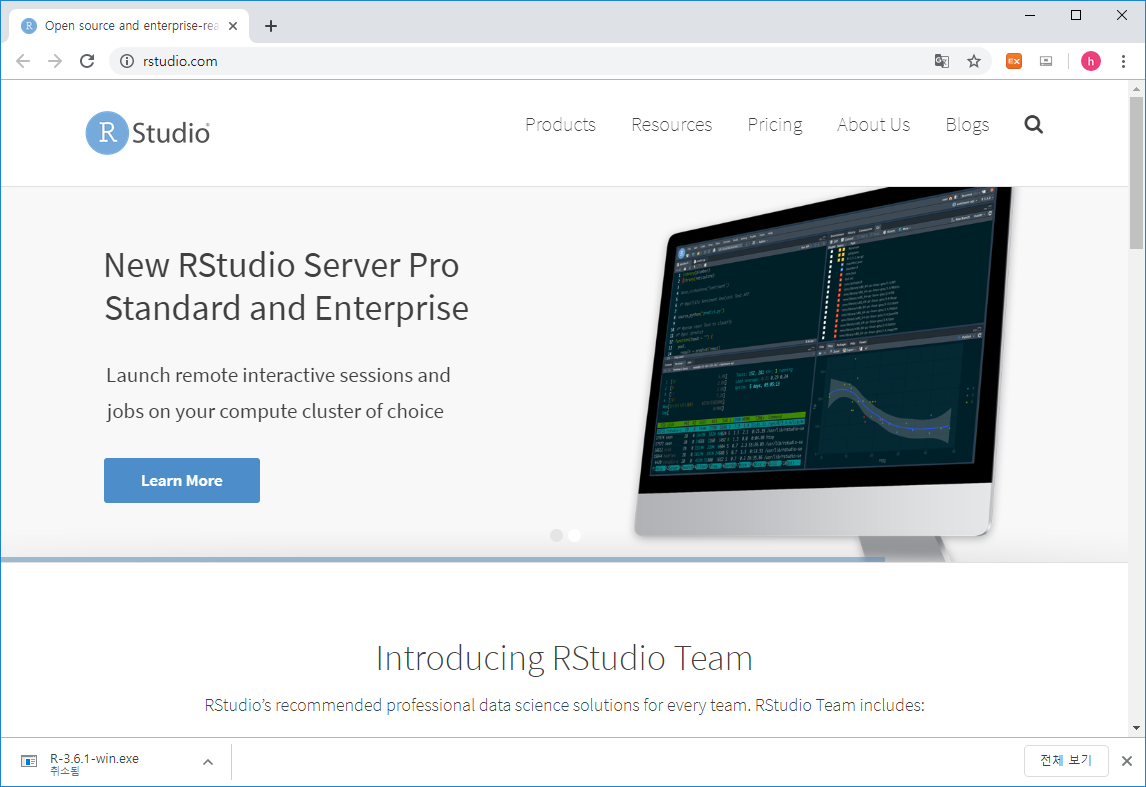
\includegraphics{images/01/01-06.PNG}
\item
  RStudio Desktop 선택
  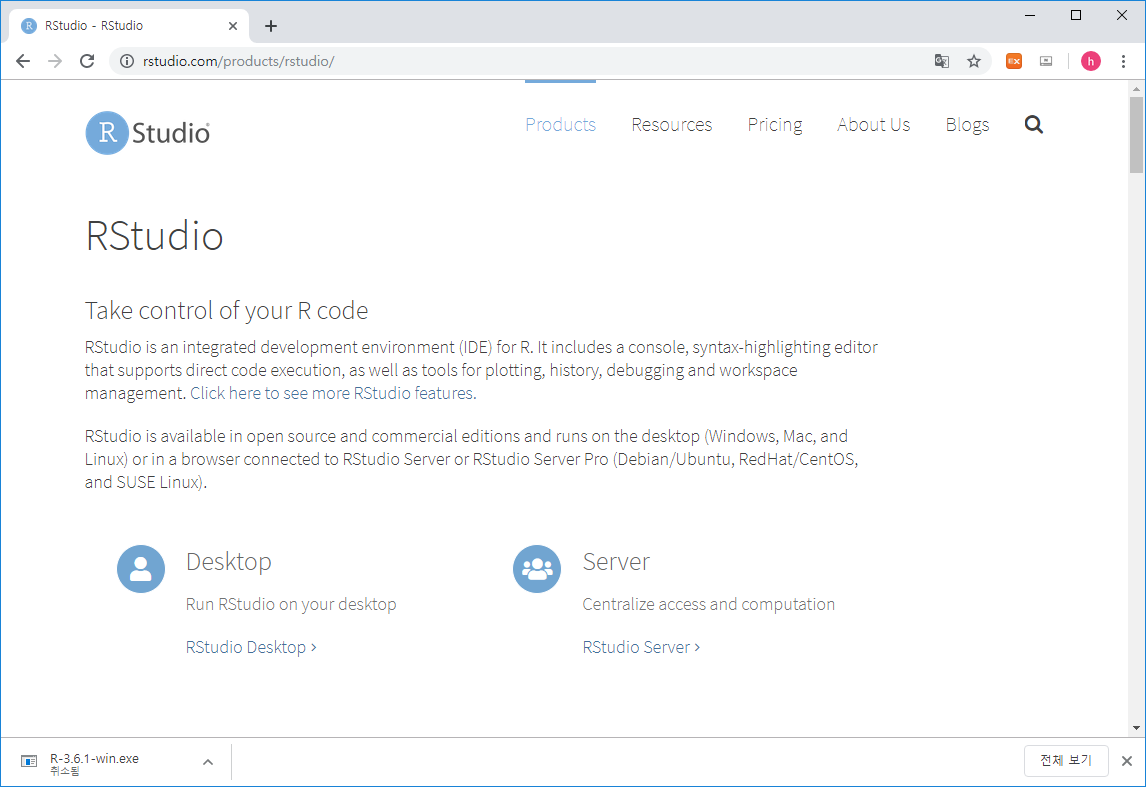
\includegraphics{images/01/01-07.PNG}
\item
  Download RStudio Desktop 클릭
  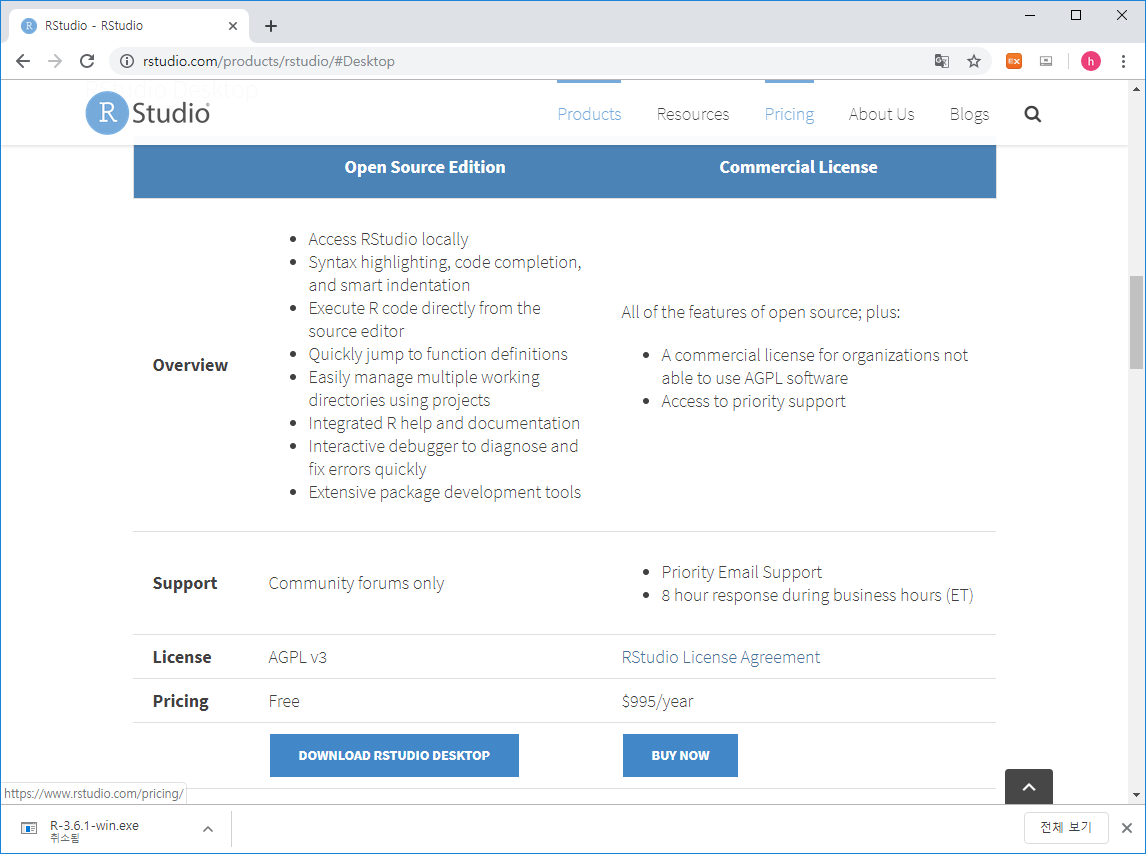
\includegraphics{images/01/01-08.PNG}
\item
  RStudio Desktop Free 버전의 Download를 선택하고
  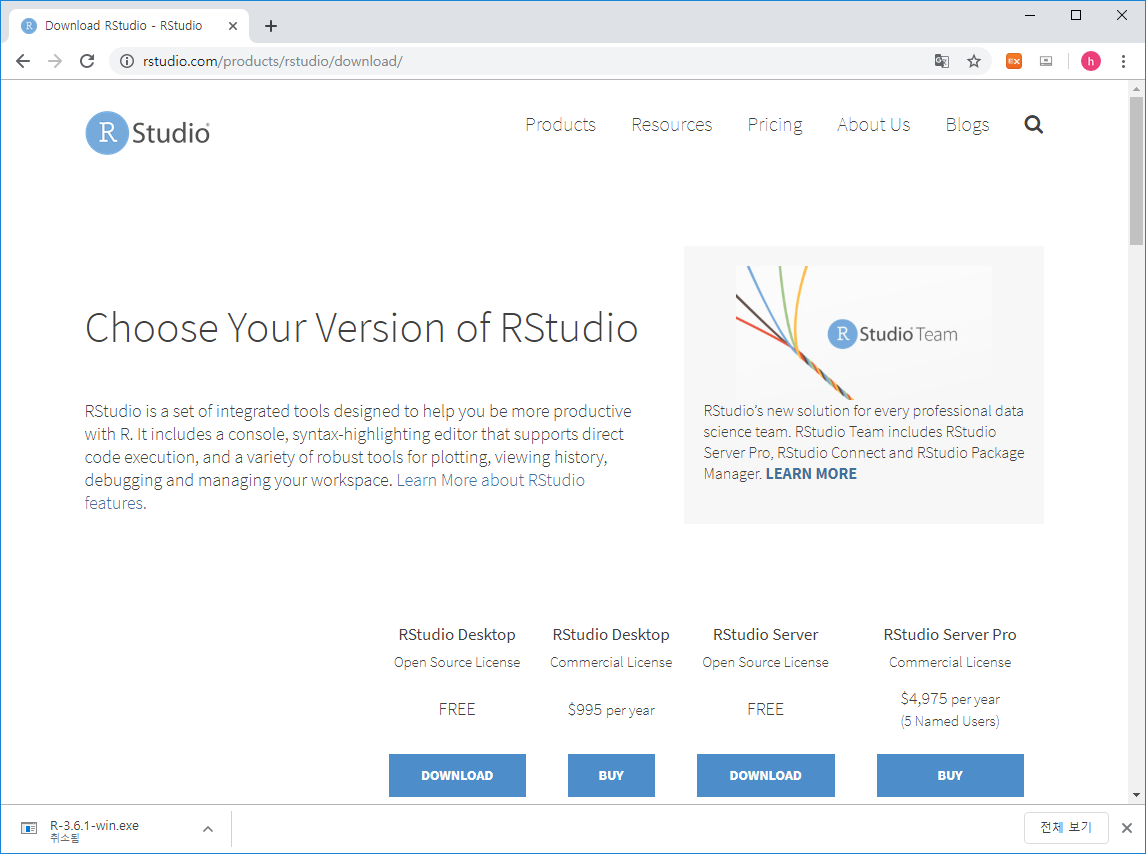
\includegraphics{images/01/01-09.PNG}
\item
  Download RStudio for Windows (2020.03현재 version 1.2.5033) 클릭, 다운로드. 로컬 컴퓨터에 다운로드된 RStudio-1.2.5033.exe를 실행하고 설치 가이드에 따라 설치 완료합니다.
  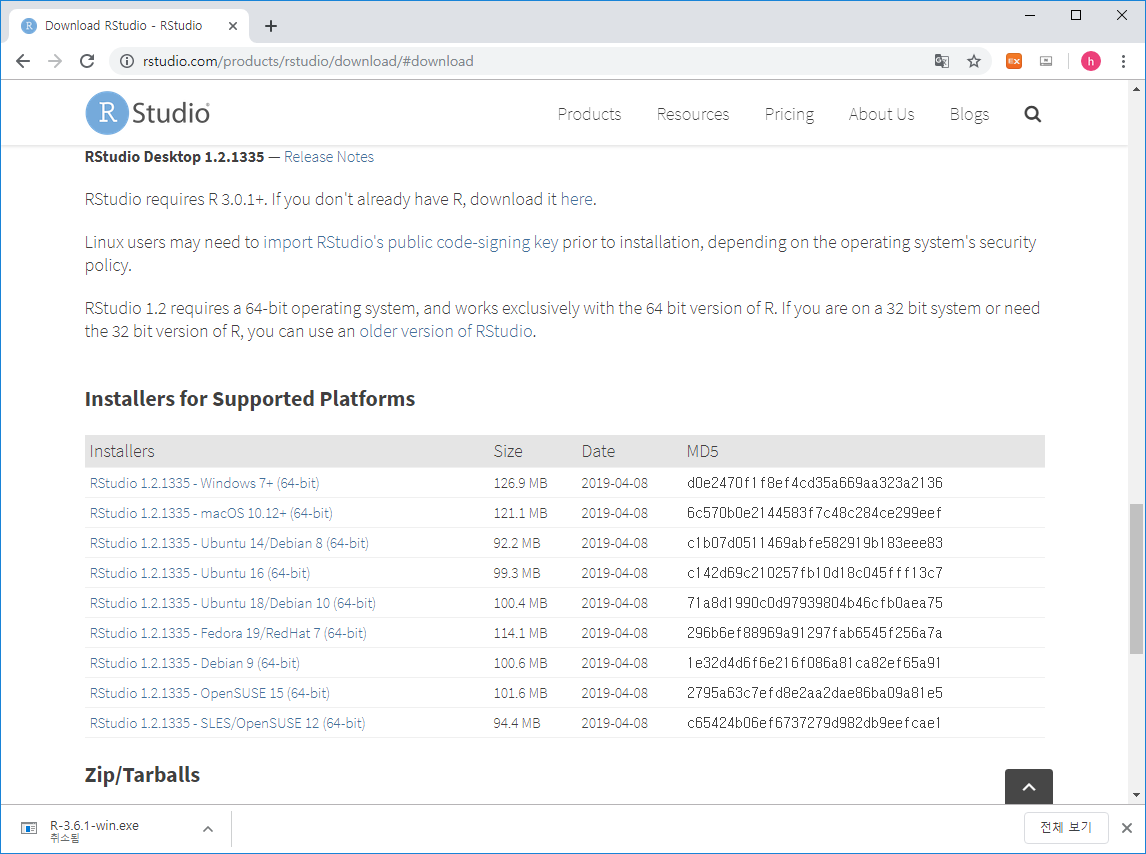
\includegraphics{images/01/01-10.PNG}
\end{itemize}

\hypertarget{rstudio-interface}{%
\section{Rstudio interface}\label{rstudio-interface}}

\begin{itemize}
\tightlist
\item
  아래 그림의 좌측 상단의 공간은 코드편집창, 좌측 하단은 콘솔창 입니다.
  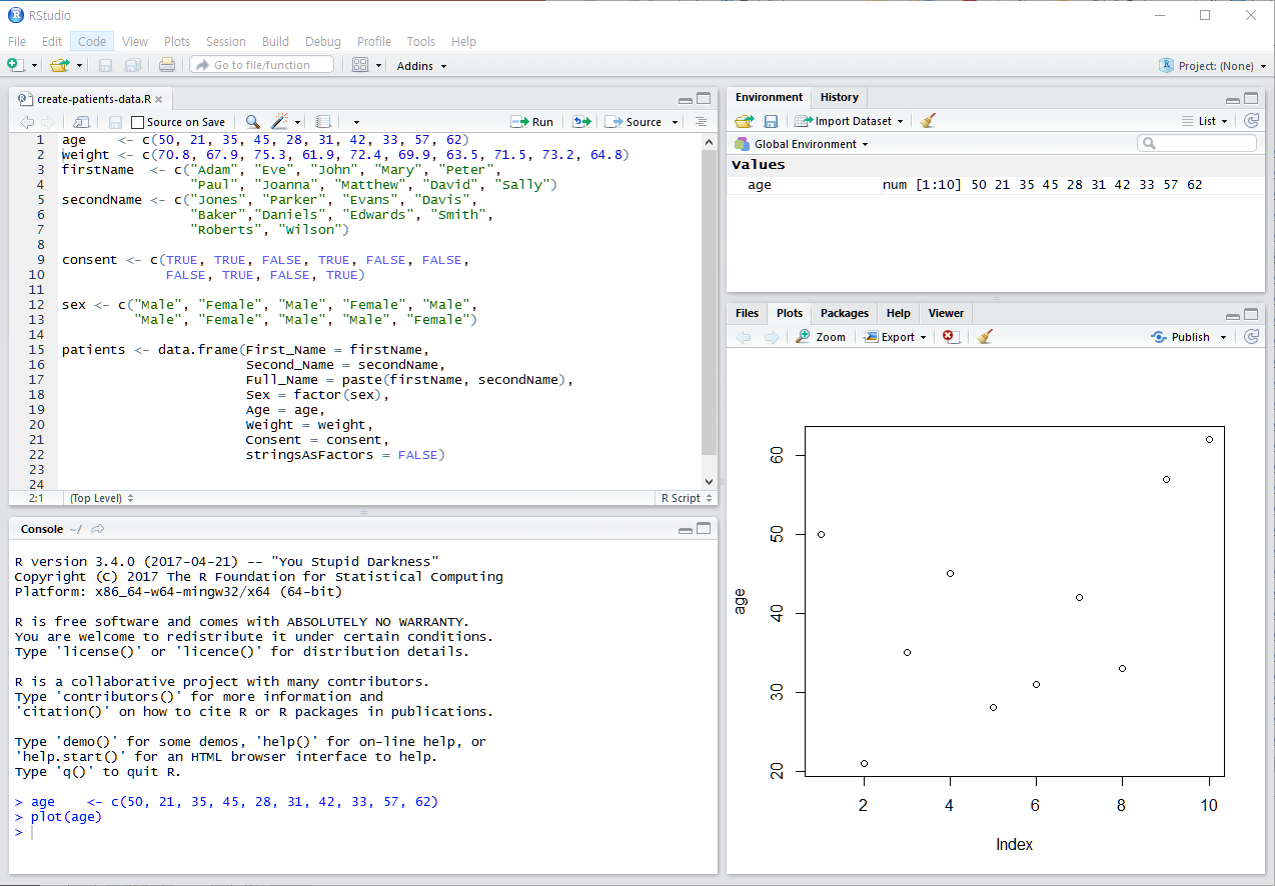
\includegraphics{images/01/01-11.PNG}
\end{itemize}

\hypertarget{keyboard-shortcuts}{%
\section{Keyboard shortcuts}\label{keyboard-shortcuts}}

\begin{itemize}
\tightlist
\item
  참고사이트

  \begin{itemize}
  \tightlist
  \item
    \url{https://support.rstudio.com/hc/en-us/articles/200711853-Keyboard-Shortcuts}
  \item
    Tools --\textgreater{} Keyboard shortcut Quick Reference (\texttt{Alt\ +\ Shift\ +\ K})
  \end{itemize}
\item
  코드편집창 이동 (\texttt{Ctrl+1}) 콘솔창 이동(\texttt{Ctrl+2})
\item
  한 줄 실행 (\texttt{Ctrl+Enter})
\item
  주석처리 (\texttt{Ctrl\ +\ Shift\ +\ C})

  \begin{itemize}
  \tightlist
  \item
    또는 \texttt{\#}으로 시작하는 라인
  \end{itemize}
\item
  실습

  \begin{itemize}
  \tightlist
  \item
    코드편집창에서 다음 입력
  \item
    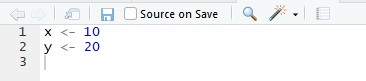
\includegraphics{images/01/01-14.PNG}\\
  \item
    단축키 \texttt{Ctrl\ +\ enter}로 코드 실행
  \item
    단축키 \texttt{Ctrl\ +\ 2}로 커서 콘솔창으로 이동
  \item
    \texttt{x}값 \texttt{x+y}값 확인
  \item
    단축키 \texttt{Ctrl\ +\ 1}로 코드편집창 이동
  \item
    단축키 \texttt{Ctrl\ +\ Shift\ +\ C} 사용
  \end{itemize}
\end{itemize}

\begin{Shaded}
\begin{Highlighting}[]
\CommentTok{\# x \textless{}{-} 10}
\CommentTok{\# y \textless{}{-} 20}
\end{Highlighting}
\end{Shaded}

\hypertarget{set-working-directory}{%
\section{Set working directory}\label{set-working-directory}}

시작 전 항상 작업 디렉토리 설정. 예를 들어 c:~아래 새로운 디렉토리 rprog2020 을 만들고 작업공간으로 설정

\begin{Shaded}
\begin{Highlighting}[]
\FunctionTok{getwd}\NormalTok{()}
\FunctionTok{dir}\NormalTok{()}
\FunctionTok{setwd}\NormalTok{(}\StringTok{"C:}\SpecialCharTok{\textbackslash{}\textbackslash{}}\StringTok{rprog2020"}\NormalTok{)}
\FunctionTok{getwd}\NormalTok{()}
\FunctionTok{dir}\NormalTok{()}
\end{Highlighting}
\end{Shaded}

또는 아래와 같이 RStudio 메뉴 에서 설정

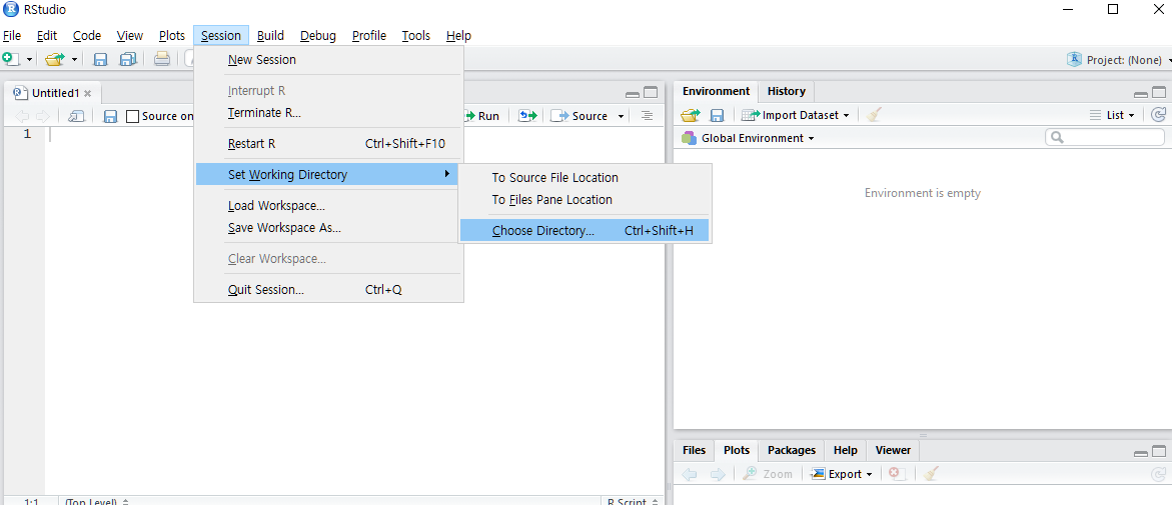
\includegraphics{images/01/01-12.PNG}

\hypertarget{hello-world}{%
\section{Hello world}\label{hello-world}}

\begin{Shaded}
\begin{Highlighting}[]
\NormalTok{mystring }\OtherTok{\textless{}{-}} \StringTok{"Hello }\SpecialCharTok{\textbackslash{}n}\StringTok{ world!"}
\FunctionTok{cat}\NormalTok{(mystring)}
\FunctionTok{print}\NormalTok{(mystring)}
\end{Highlighting}
\end{Shaded}

\hypertarget{help}{%
\section{Help}\label{help}}

R의 장점 중 하나로 방대한 양의 도움말 페이지가 제공됩니다. \texttt{?} 명령을 사용하면 되며 구글이나 웹에서도 도움을 얻을 수 있습니다.

\begin{Shaded}
\begin{Highlighting}[]
\NormalTok{?cat}
\NormalTok{?print}
\NormalTok{?mean}
\FunctionTok{help}\NormalTok{(}\StringTok{"mean"}\NormalTok{)}
\FunctionTok{example}\NormalTok{(}\StringTok{"mean"}\NormalTok{)}
\FunctionTok{help.search}\NormalTok{(}\StringTok{"mean"}\NormalTok{)}
\FunctionTok{help}\NormalTok{(}\AttributeTok{package=}\StringTok{"MASS"}\NormalTok{)}
\end{Highlighting}
\end{Shaded}

\hypertarget{rstudio-workspace}{%
\section{RStudio workspace}\label{rstudio-workspace}}

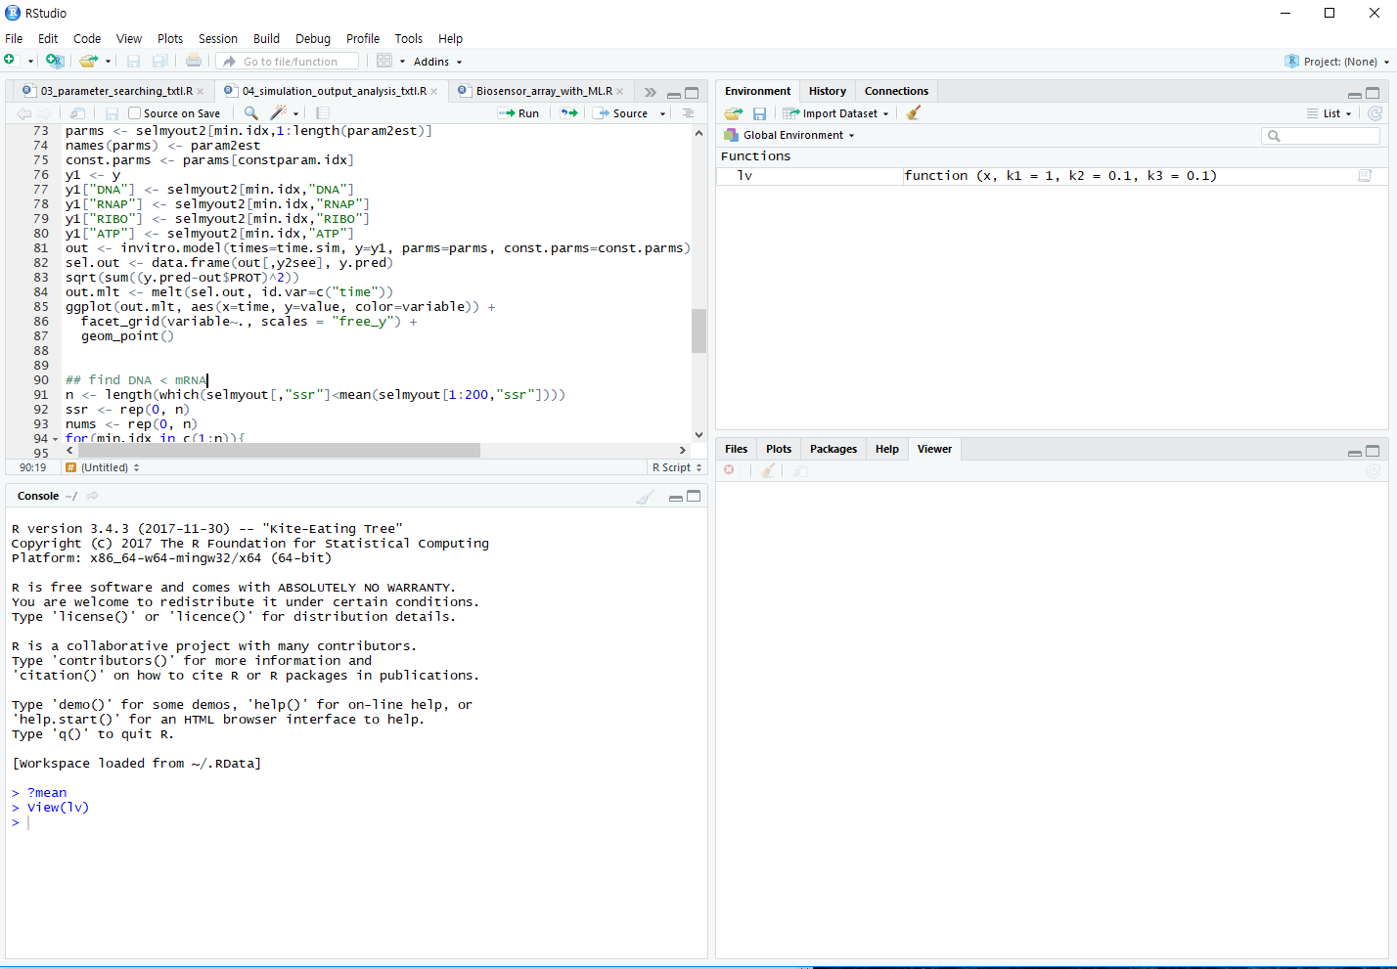
\includegraphics{images/01/01-17.PNG}
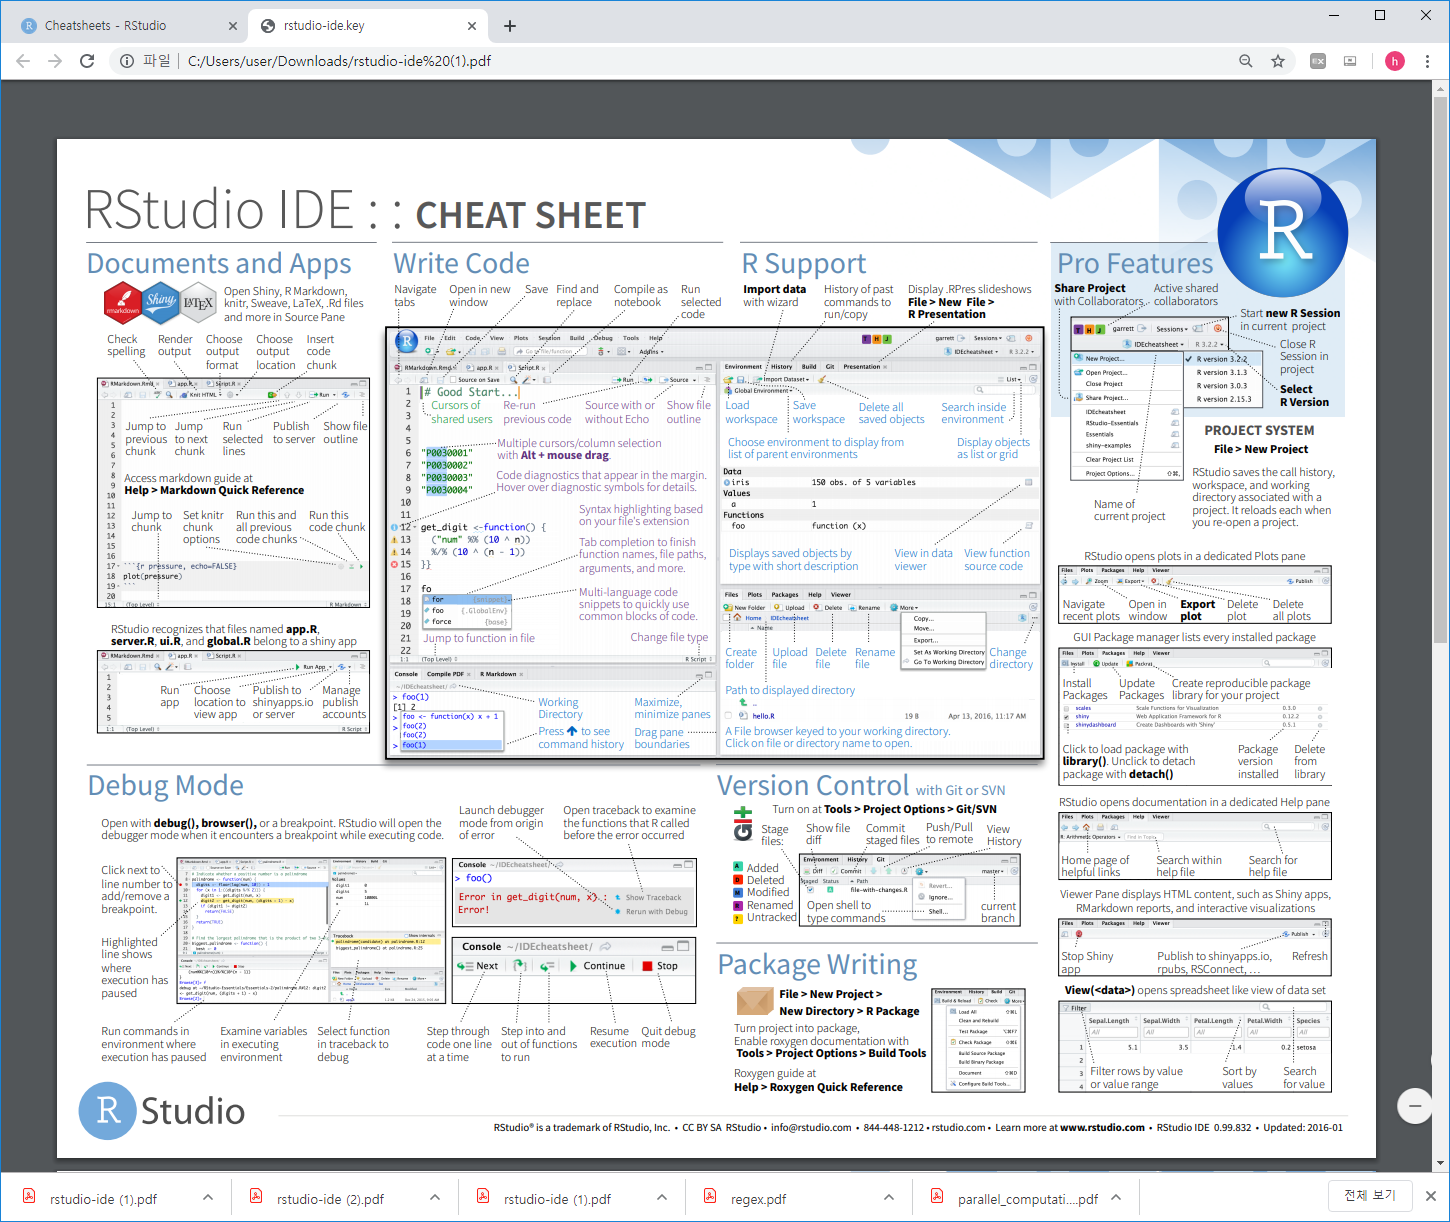
\includegraphics{images/01/rstudio-ide-1.png}
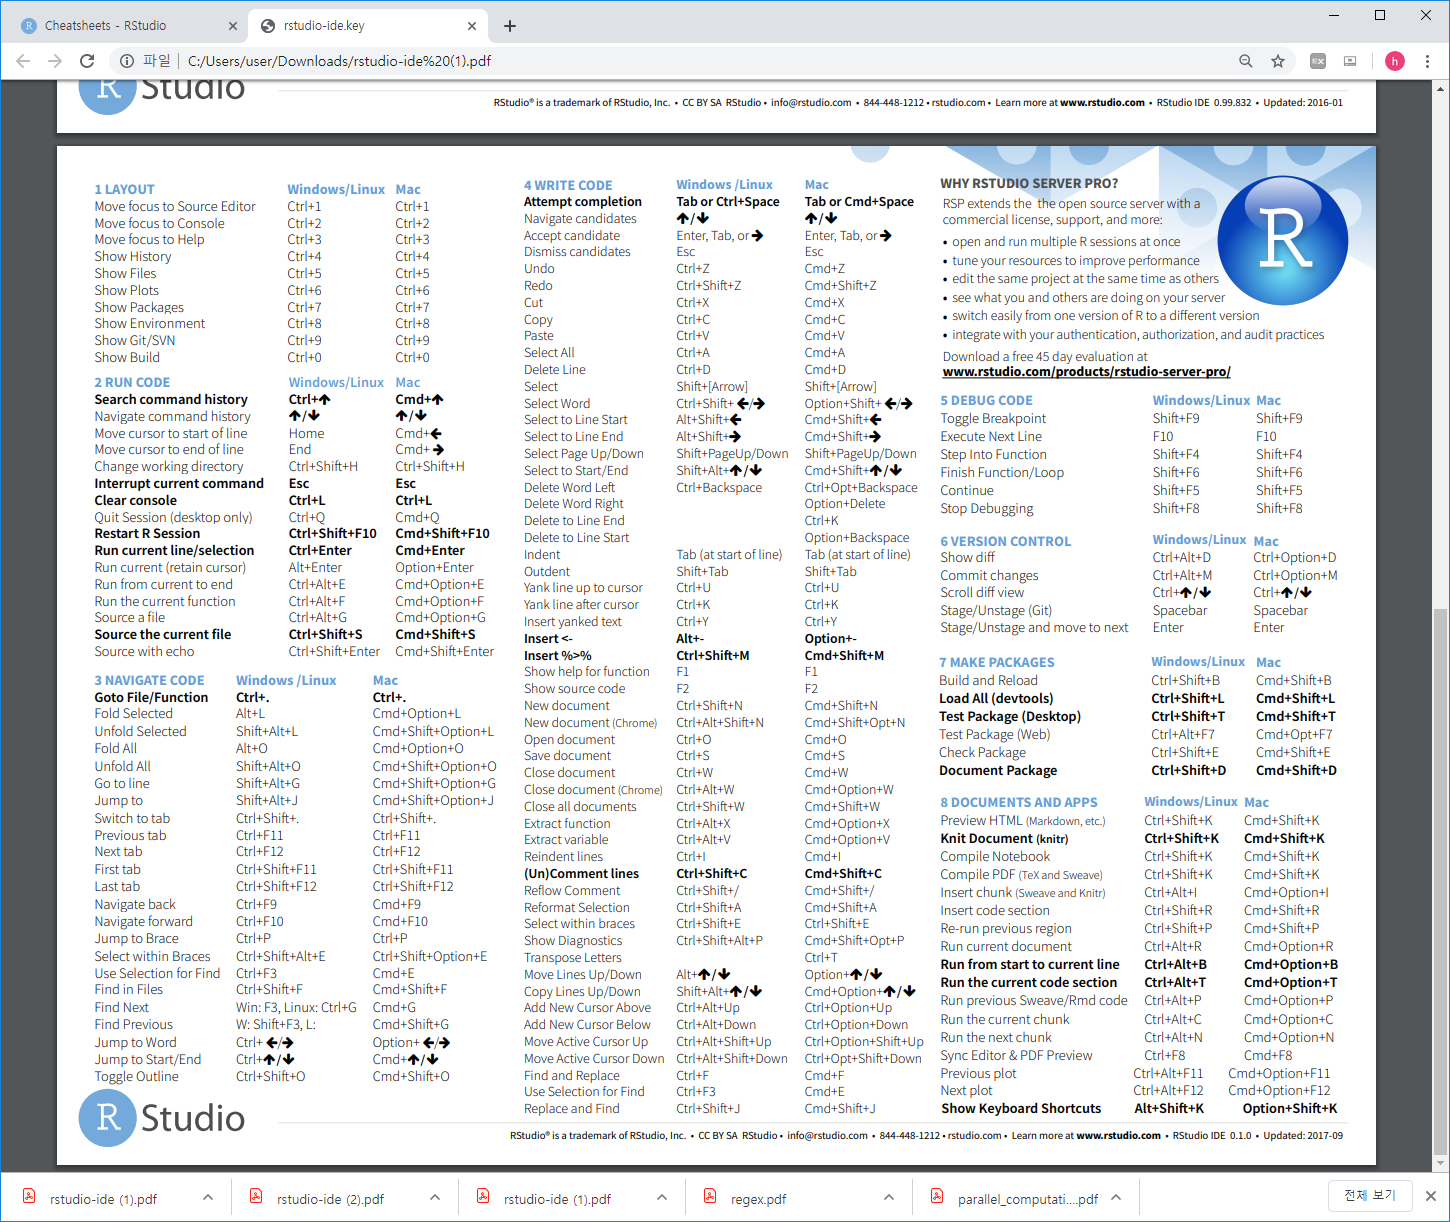
\includegraphics{images/01/rstudio-ide-2.png}

\hypertarget{r-packages}{%
\section{R packages}\label{r-packages}}

R은 ``package''라 불리우는 다양한 함수 라이브러리를 사용할 수 있습니다. 예를 들어 \texttt{sum()} 이나 \texttt{sd()}와 같은 함수는 \texttt{stats}이라는 패키지에서 구현된 함수 입니다. 이러한 패키지는 인터넷의 \texttt{repository}에서 구할 수 있으며 대표적으로 The Comprehensive R Archive Network (CRAN) \url{http://cran.r-project.org/web/views/} 와 생물학자를 위한 Bioconductor specialised in genomics \url{http://www.bioconductor.org/packages/release/BiocViews.html\#___Software} 가 있습니다. 이러한 패키지의 설치는 아래와 같이 RStudio를 이용하거나 콘솔창에서 \texttt{install.packages()} 함수를 이용할 수 있습니다.

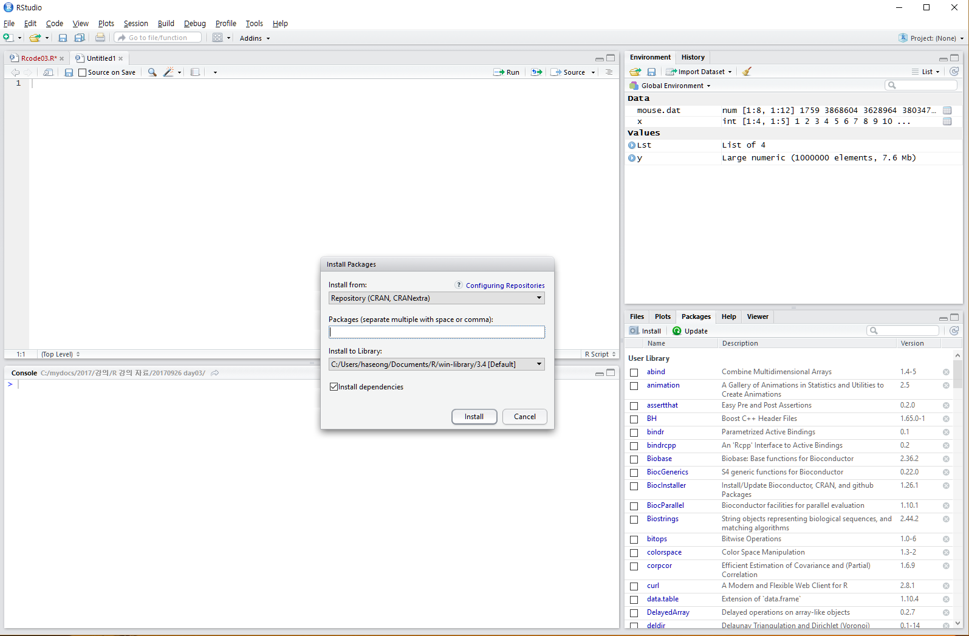
\includegraphics{images/01/01-18.png}

\begin{itemize}
\tightlist
\item
  UsingR package installation
\end{itemize}

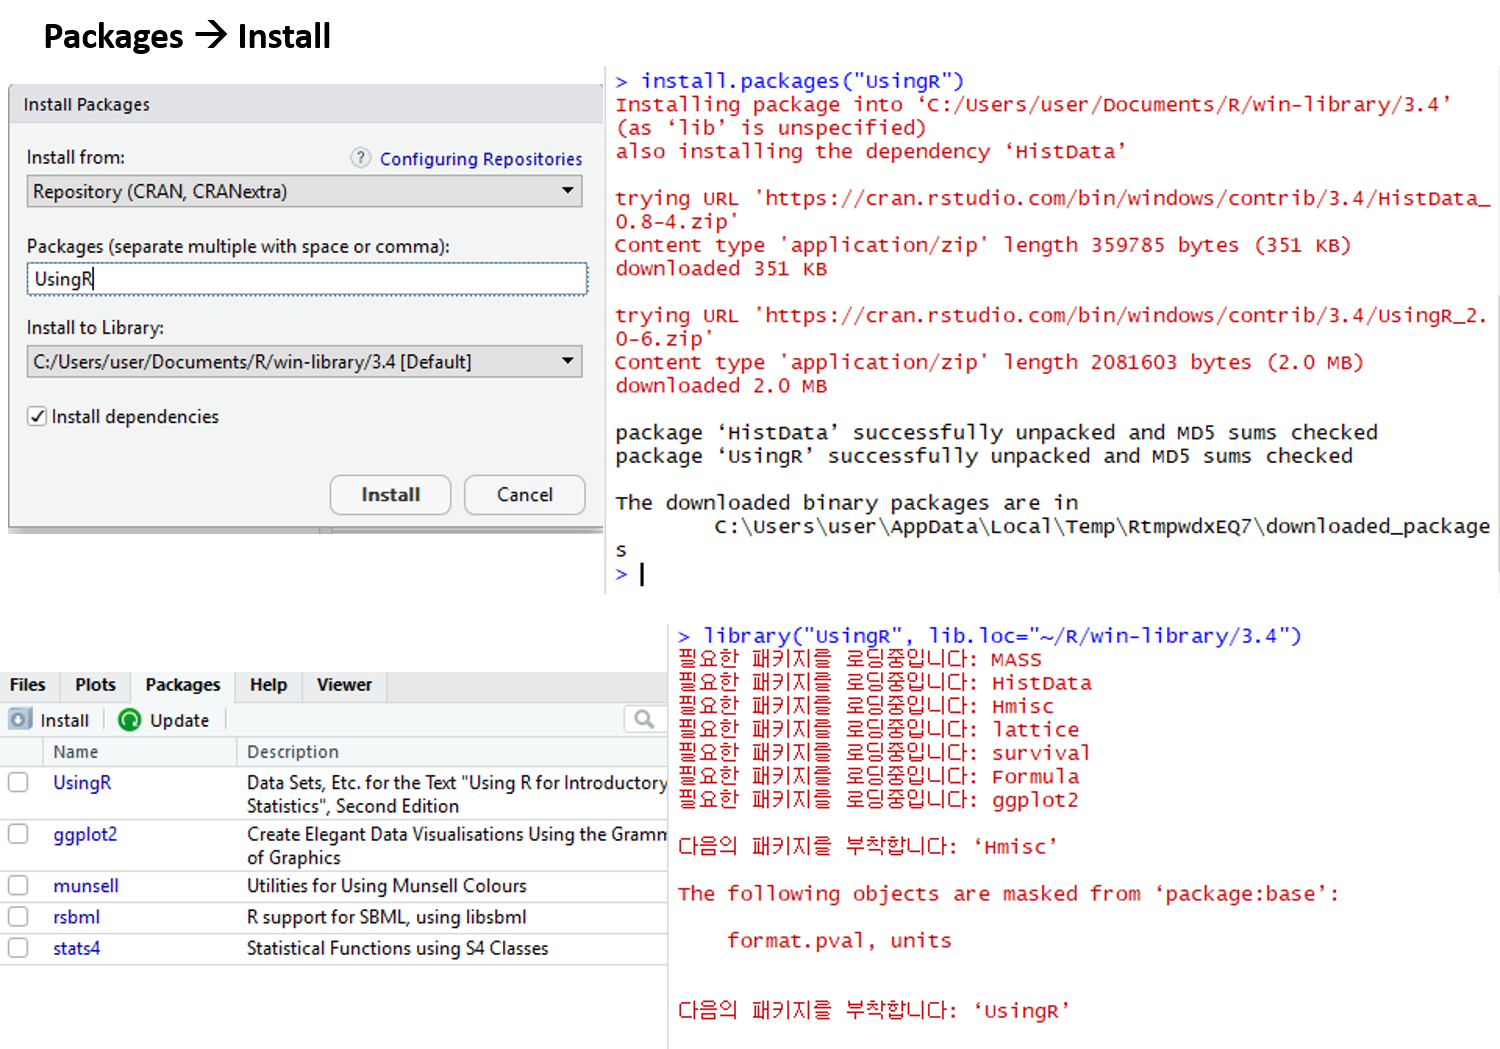
\includegraphics{images/01/01-19.png}

패키지를 설치하고 사용하기 위해서는 \texttt{library()} 함수를 사용해서 미리 loading 해 두어야 합니다. 한 번 로딩으로 작업 세션이 끝날때까지 관련된 함수를 사용할 수 있으나 R 세션이나 RStudio를 재시작 할 경우 다시 로딩해야 사용할 수 있습니다.

\begin{Shaded}
\begin{Highlighting}[]
\FunctionTok{library}\NormalTok{(UsingR)}
\end{Highlighting}
\end{Shaded}

\begin{itemize}
\tightlist
\item
  R 설치 디렉토리
\item
  R 패키지 설치 디렉토리
\end{itemize}

\begin{Shaded}
\begin{Highlighting}[]
\FunctionTok{.libPaths}\NormalTok{()}
\FunctionTok{path.package}\NormalTok{()}
\end{Highlighting}
\end{Shaded}

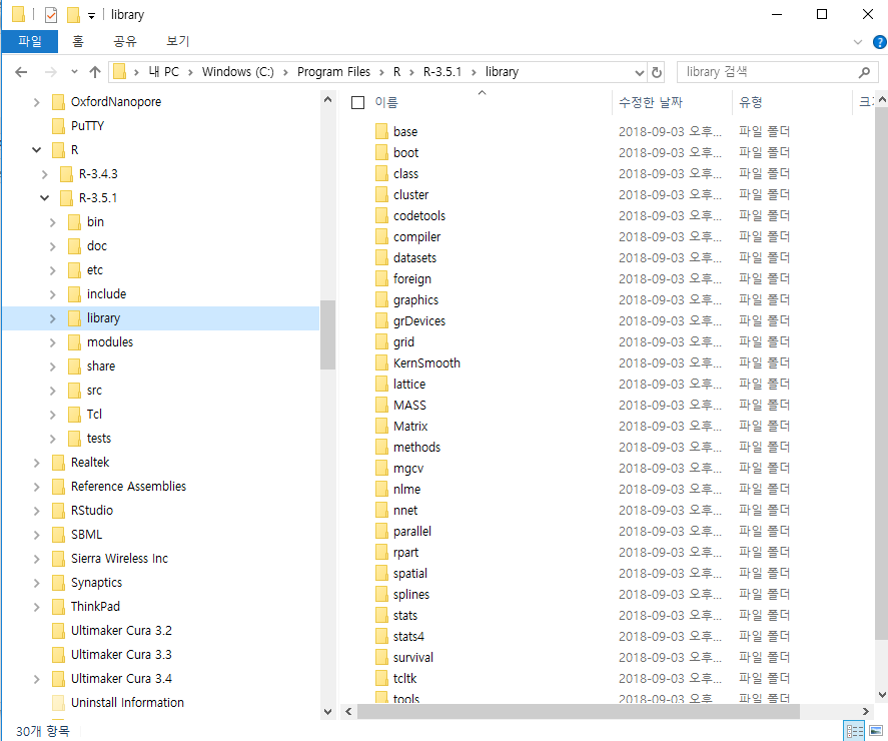
\includegraphics{images/01/01-20.png}

\hypertarget{data-sets}{%
\section{Data sets}\label{data-sets}}

대부분의 패키지는 함수와 함께 관련된 도움말, 예제, 그리고 데이터셋을 같이 제공해 줍니다. \texttt{library()} 함수를 사용할 때 자동으로 같이 로딩이 되며 \texttt{data()} 함수를 사용해서 사용자 작업공간에 복사본을 만들어서 사용할 수 있습니다.

\begin{Shaded}
\begin{Highlighting}[]
\FunctionTok{head}\NormalTok{(rivers)}
\FunctionTok{length}\NormalTok{(rivers)}
\FunctionTok{class}\NormalTok{(rivers)}
\FunctionTok{data}\NormalTok{(rivers)}
\FunctionTok{data}\NormalTok{(}\AttributeTok{package=}\StringTok{"UsingR"}\NormalTok{)}
\FunctionTok{library}\NormalTok{(HistData)}
\FunctionTok{head}\NormalTok{(Cavendish)}
\FunctionTok{str}\NormalTok{(Cavendish)}
\FunctionTok{head}\NormalTok{(Cavendish}\SpecialCharTok{$}\NormalTok{density2)}
\FunctionTok{data}\NormalTok{(}\AttributeTok{package=}\StringTok{"HistData"}\NormalTok{)}
\end{Highlighting}
\end{Shaded}

\hypertarget{cheatsheet}{%
\section{Cheatsheet}\label{cheatsheet}}

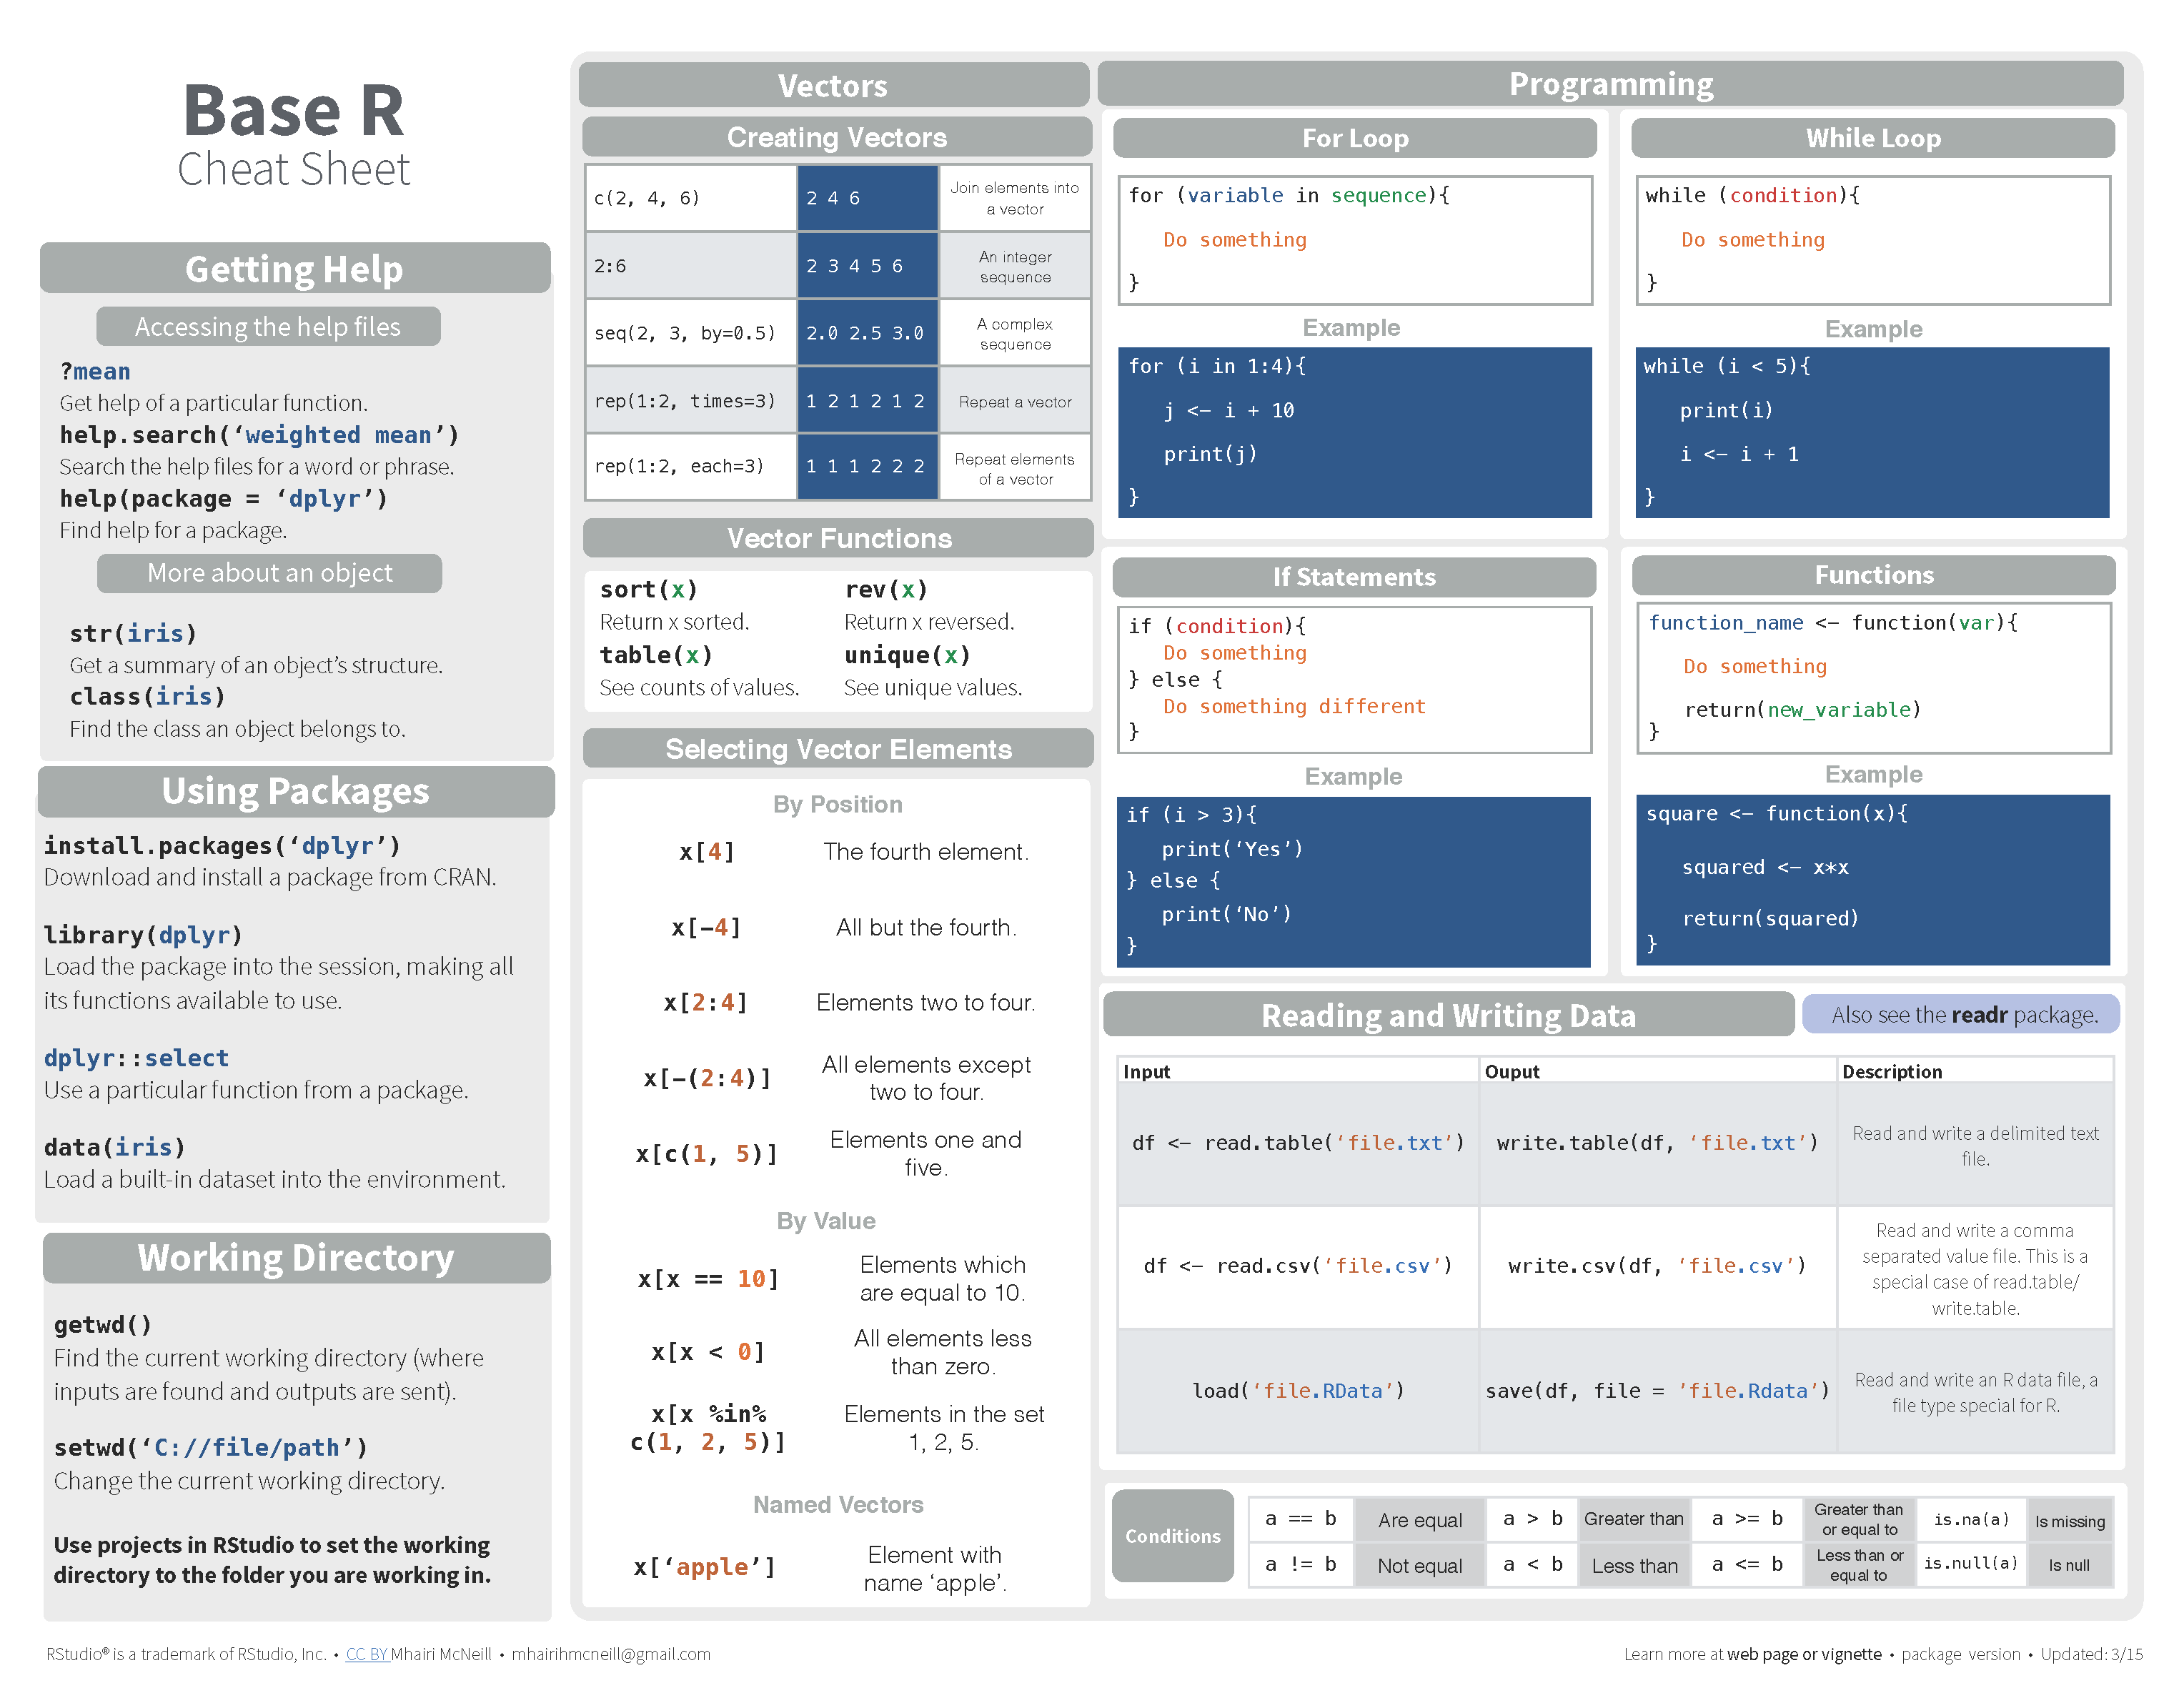
\includegraphics{images/01/base-r_1.png}
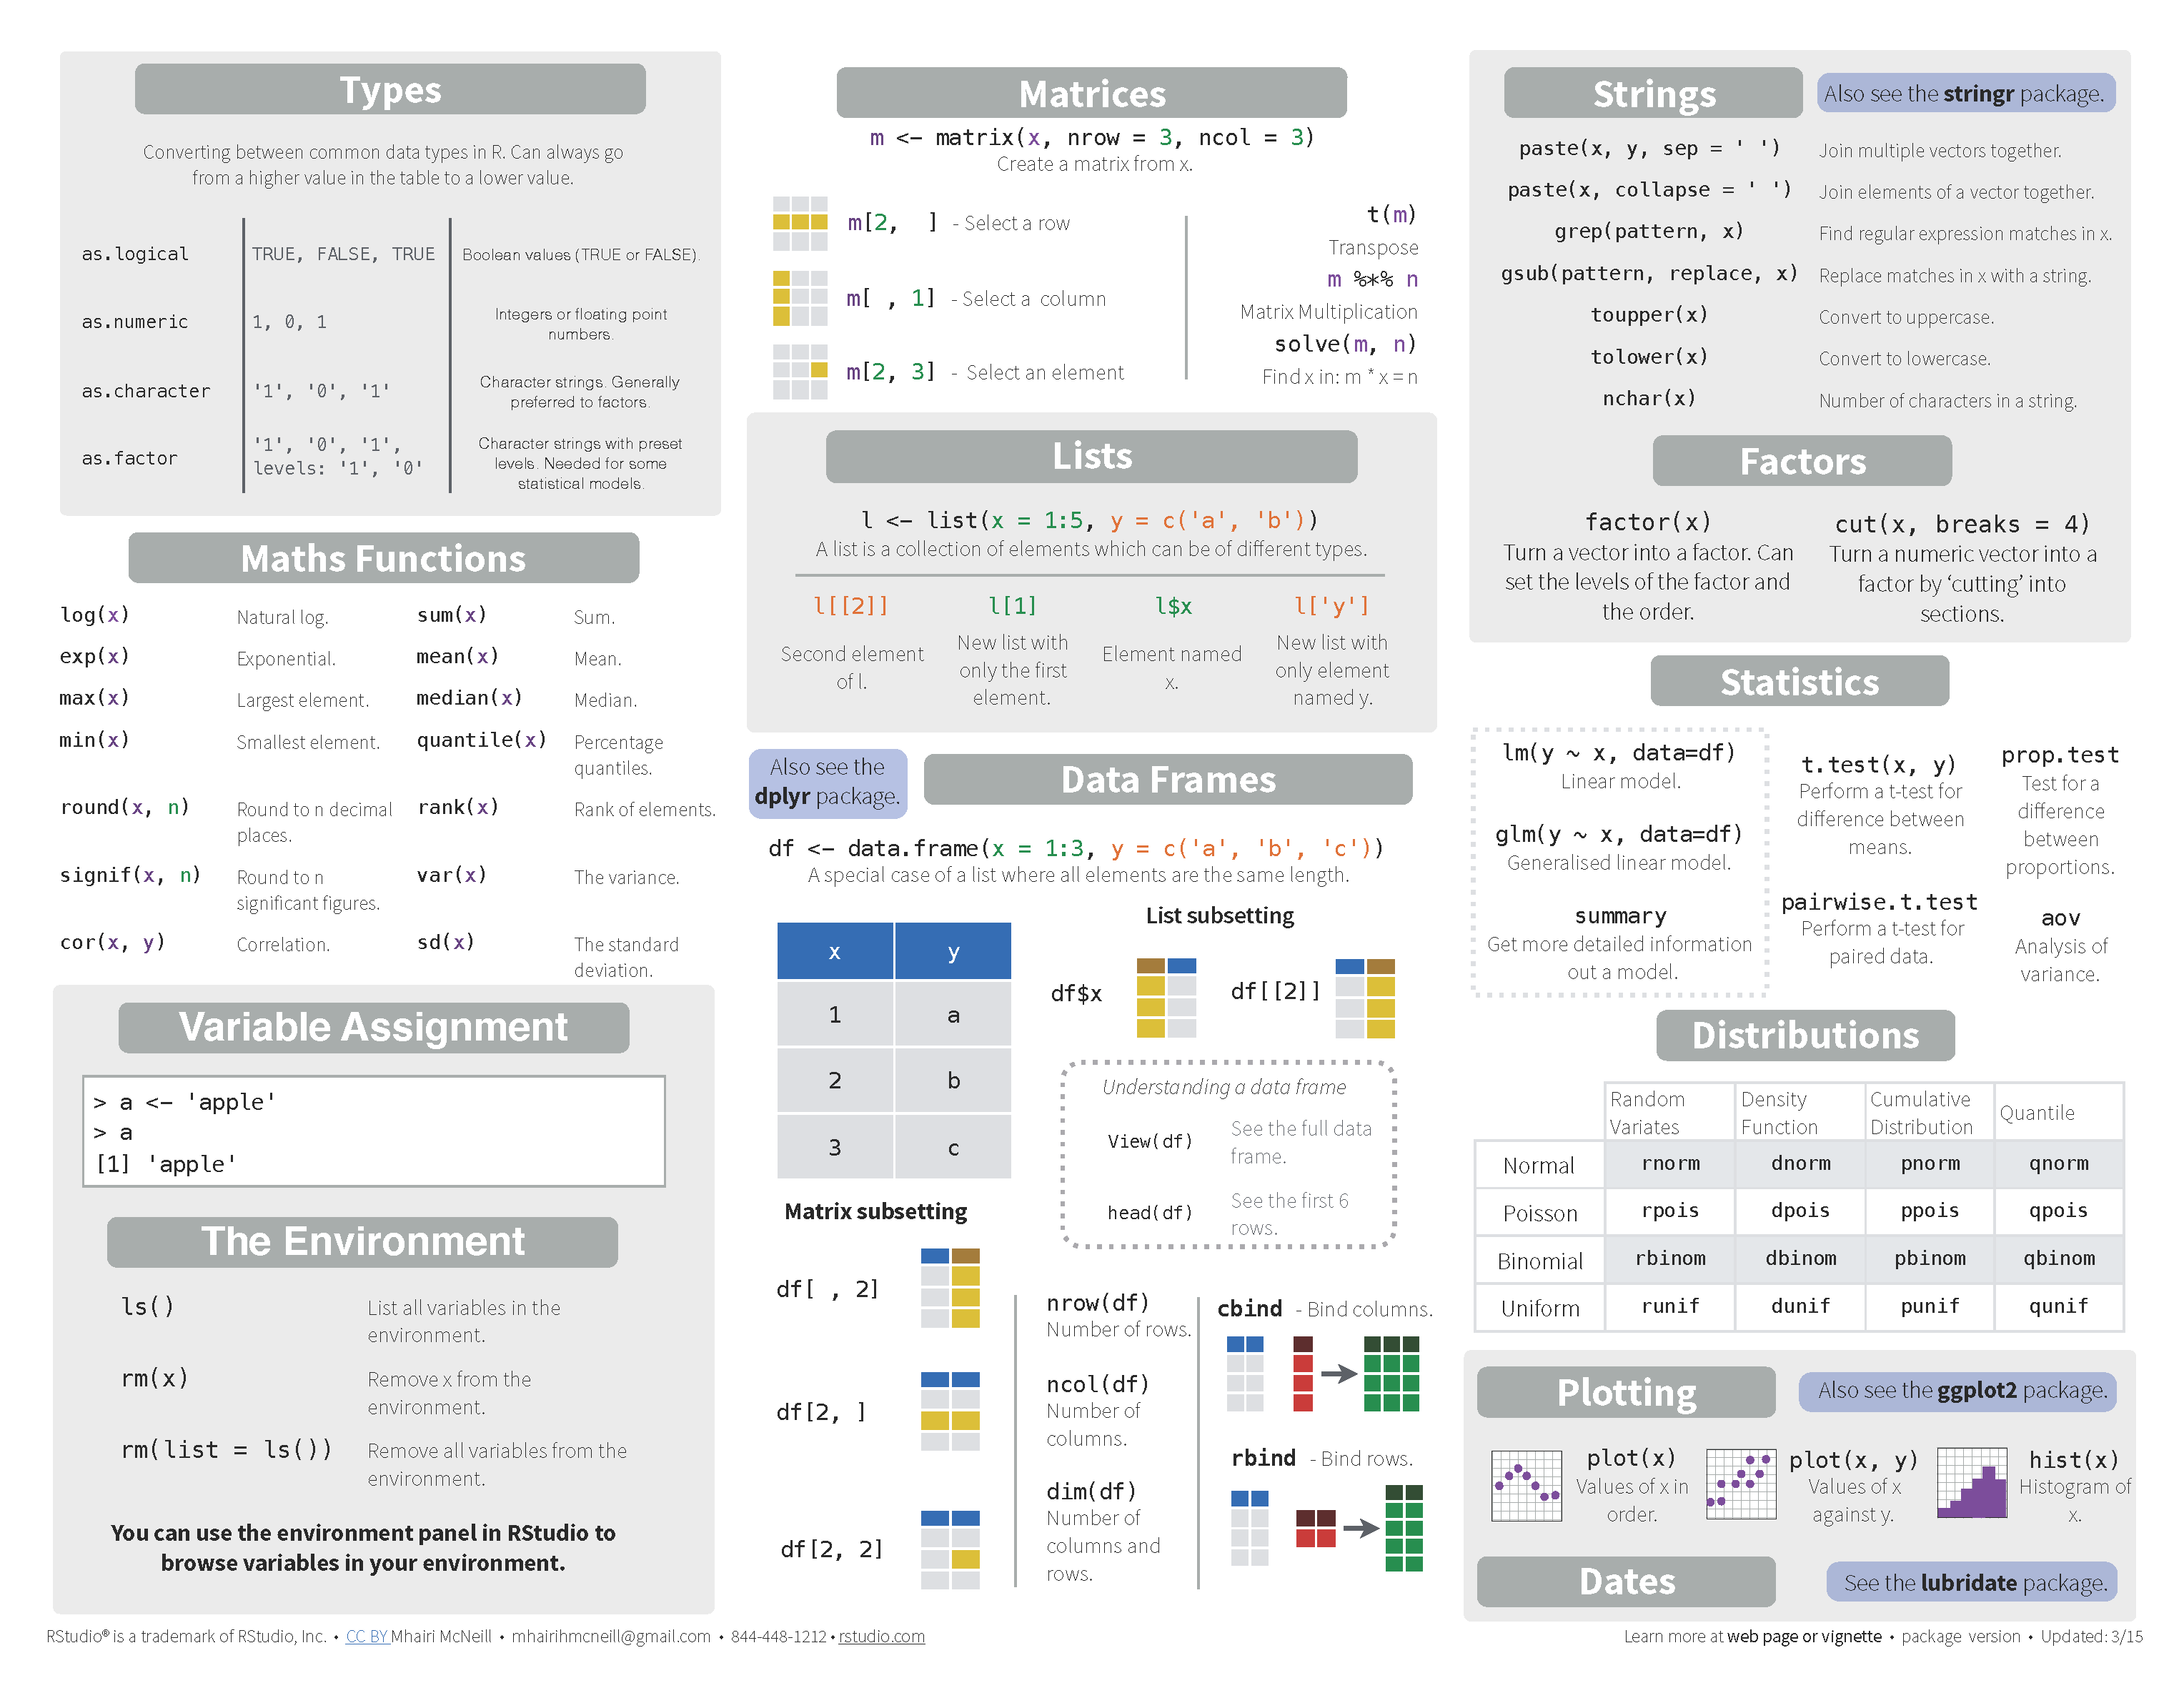
\includegraphics{images/01/base-r_2.png}

\begin{center}\rule{0.5\linewidth}{0.5pt}\end{center}

이 저작물은 크리에이티브 커먼즈 저작자표시-비영리-변경금지 4.0 국제 라이선스에 따라 이용할 수 있습니다.

  \bibliography{book.bib,packages.bib}

\end{document}
